%!TEX root = ../my_thesis.tex
\section{Systematics}
\label{sec:systematics}

The identified systematic uncertainties are listed in
Table~\ref{tab:summarySyst} in decreasing order of their size.
Their quadratic sum is \Sfsyst~and \Sfbsyst~for $S_{f}$ and $S_{\bar f}$, respectively.
A description of each systematic effect  is given in the following subsections.
The ``fit biases'' are the residuals observed in the Monte Carlo bootstrap study discussed
in Sec.~\ref{sec:mcbootstrap}.

\begin{table}[htbp]
	\centering
	\caption{Systematic uncertainties on the \CP~parameters $S_{f}$ and
	$S_{\bar f}$.}
	\begin{tabular}{lcc}
		\toprule
		Source & $S_{f}$ & $S_{\bar f}$ \\
		\midrule
		uncertainty of $\Delta m$ & \num{0.0073} & \num{0.0061} \\
        fit biases & \num{0.0068} & \num{0.0018} \\
        background subtraction  & \num{0.0042} & \num{0.0023} \\
        flavour tagging calibration models & \num{0.0011} & \num{0.0015} \\
        flavour tagging efficiency asymmetries & \num{0.0012} & \num{0.0015} \\
        PIDK efficiencies & \num{0.0008} & \num{0.0008} \\
        acceptance model & \num{0.0007} & \num{0.0007} \\
        assumption $\DG=0$ & \num{0.0007} & \num{0.0007} \\
        assumption $C_f=-C_{\bar f}=1$ & \num{0.0006} & \num{0.0006} \\
        decay time resolution & \num{0.0012} & \num{0.0008} \\
		\midrule
		total systematic uncertainty & 0.0111 & 0.0073 \\
		\midrule
		statistical uncertainties & 0.0198 & 0.0199 \\
		\bottomrule
	\end{tabular}
	\label{tab:summarySyst}
\end{table}

\subsection{Systematic uncertainties from Gaussian constraints}
\label{sec:systFromConsts}
Systematic uncertainties due to external measurements used in the PDF
are accounted for through Gaussian constraints in the likelihood. These parameters are
the mixing frequency, $\Delta m$, and the \Bz~lifetime, $\tau$.
The fit has been repeated by fixing the Gaussian-constrained parameters to their central values,
in order to not propagate the uncertainty of these parameters to the statistical uncertainties of the fit.
The statistical uncertainties of $S_{f}$ and $S_{\bar f}$ with $\Delta m$ fixed are $0.0198$ and $0.0199$, respectively, whereas the statistical correlation is $0.6$.
Considering the difference in quadrature between the uncertainty from the nominal fit and that from this fit,
the systematic uncertainty due to $\Delta m$ are $0.0073$ and $0.0061$ for $S_{f}$ and $S_{\bar f}$, respectively.
The correlation between the systematic uncertainties due to $\Delta m$ on $S_{f}$ and $S_{\bar f}$ is $-1$, as described in Appendix~\ref{app:corrSyst}.
The fit with $\tau$ fixed shows that the systematics uncertainty due to this parameter is negligible.

Systematic uncertainty associated with the $\PIDK$ efficiencies (Table~\ref{tab:pideff})
are taken into account
in the mass fit by means of Gaussian constraints on these parameters (Sec.~\ref{sec:DataMassFit}).  The mass fit is repeated by neglecting these uncertainties in the Gaussian constraints.
Then, the time fit is performed with this new set of \emph{sWeights}. The difference
in quadrature between the uncertainty from this fit and that from the nominal fit gives the systematic due to the binning scheme in the
$\PIDK$ resampling, which is $0.0008$ for both $S_{f}$ and $S_{\bar f}$.
%!TEX root = ../my_thesis.tex
\subsection{Systematic uncertainties estimated with pseudoexperiments}
\label{sec:systFromToys}

When computing the systematic uncertainties with pseudoexperiments (or \emph{toys}), a sample with the same size as the data is generated by sampling the PDF
with parameters fixed to the value found in the data fit. The values of \Sf~and \Sfb~are fixed
to those used in the generation of the Monte Carlo sample (Appendix~\ref{app:mcgen}).
In the generation of the samples
the PDF is modified to consider alternative models according to the source of systematic
uncertainty under investigation.
The generated sample is then fitted with the nominal model. For each parameter, the
mean of the distribution of the residuals from 1000 toys is taken
as a symmetric systematic uncertainty. If the mean is consistent with zero within $\pm 1~\sigma$,
the error on the mean is taken instead.
The systematic uncertainties estimated with this toy-based method are the following:
\begin{itemize}[noitemsep,topsep=0pt]
\item the flavour tagging calibration model;
\item the flavour tagging efficiency asymmetries;
\item the acceptance model;
\item the decay time resolution;
\item the assumption $C_f=-C_{\bar f}=1$;
\item the assumption $\DG=0$.
\end{itemize}

%-------------------------------------------------------------------------------
\subsubsection{Flavour tagging calibration model}
\label{sec:syst_toys_calibmodel}

Toys are generated using for the SS calibration the nominal model with a first order polynomial, and
for the OS the model is reduced by one degree as compared to the nominal one. In the fit,
the calibration models of both taggers are increased by one degree compared to what was used in the generation step.
The distribution of the residuals of \Sf~and \Sfb~are shown in Fig.~\ref{fig:FTSystToys}.
The residuals are not compatible with zero and therefore they are assigned as systematic uncertainties.
\begin{figure}[t]
	\begin{center}
		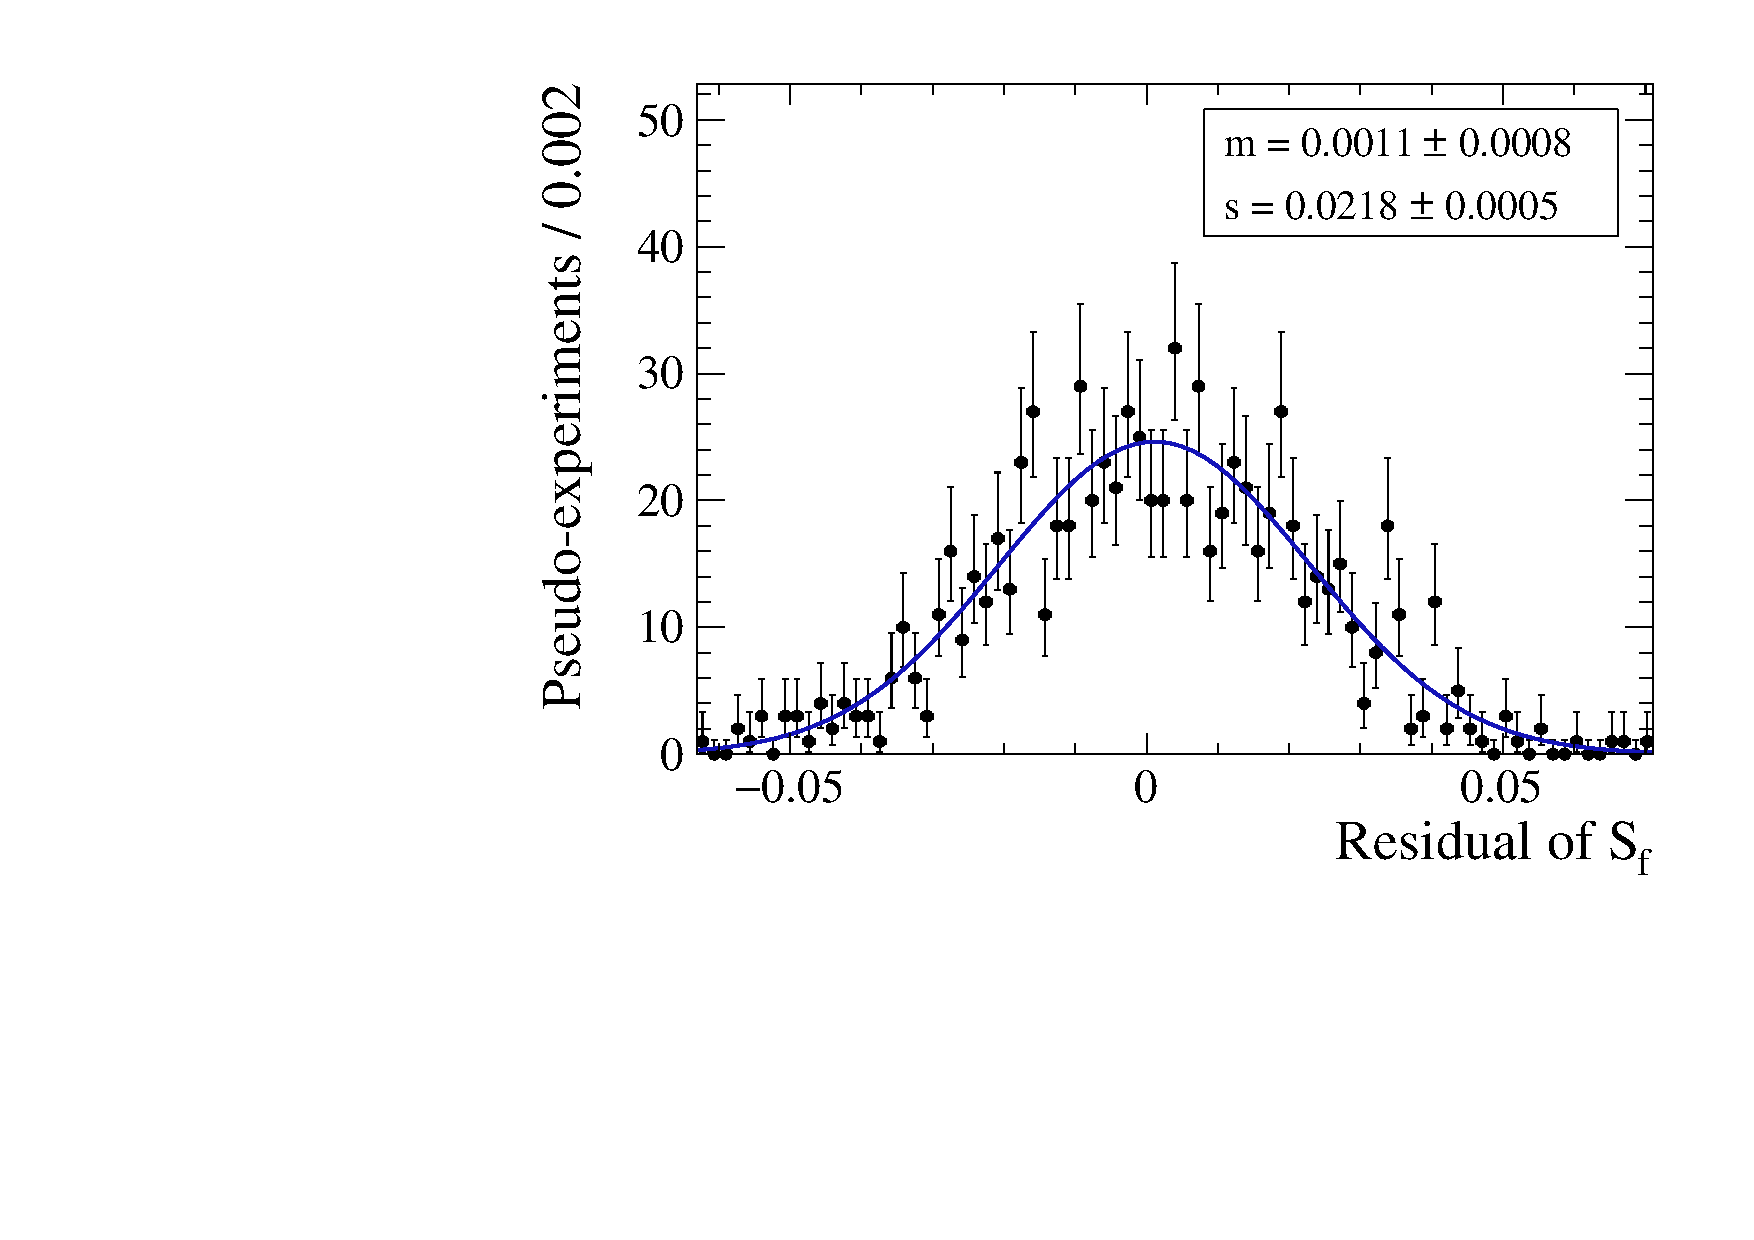
\includegraphics[width=0.4\textwidth]{06Systematics/figs/FT_Sf_res.pdf}
		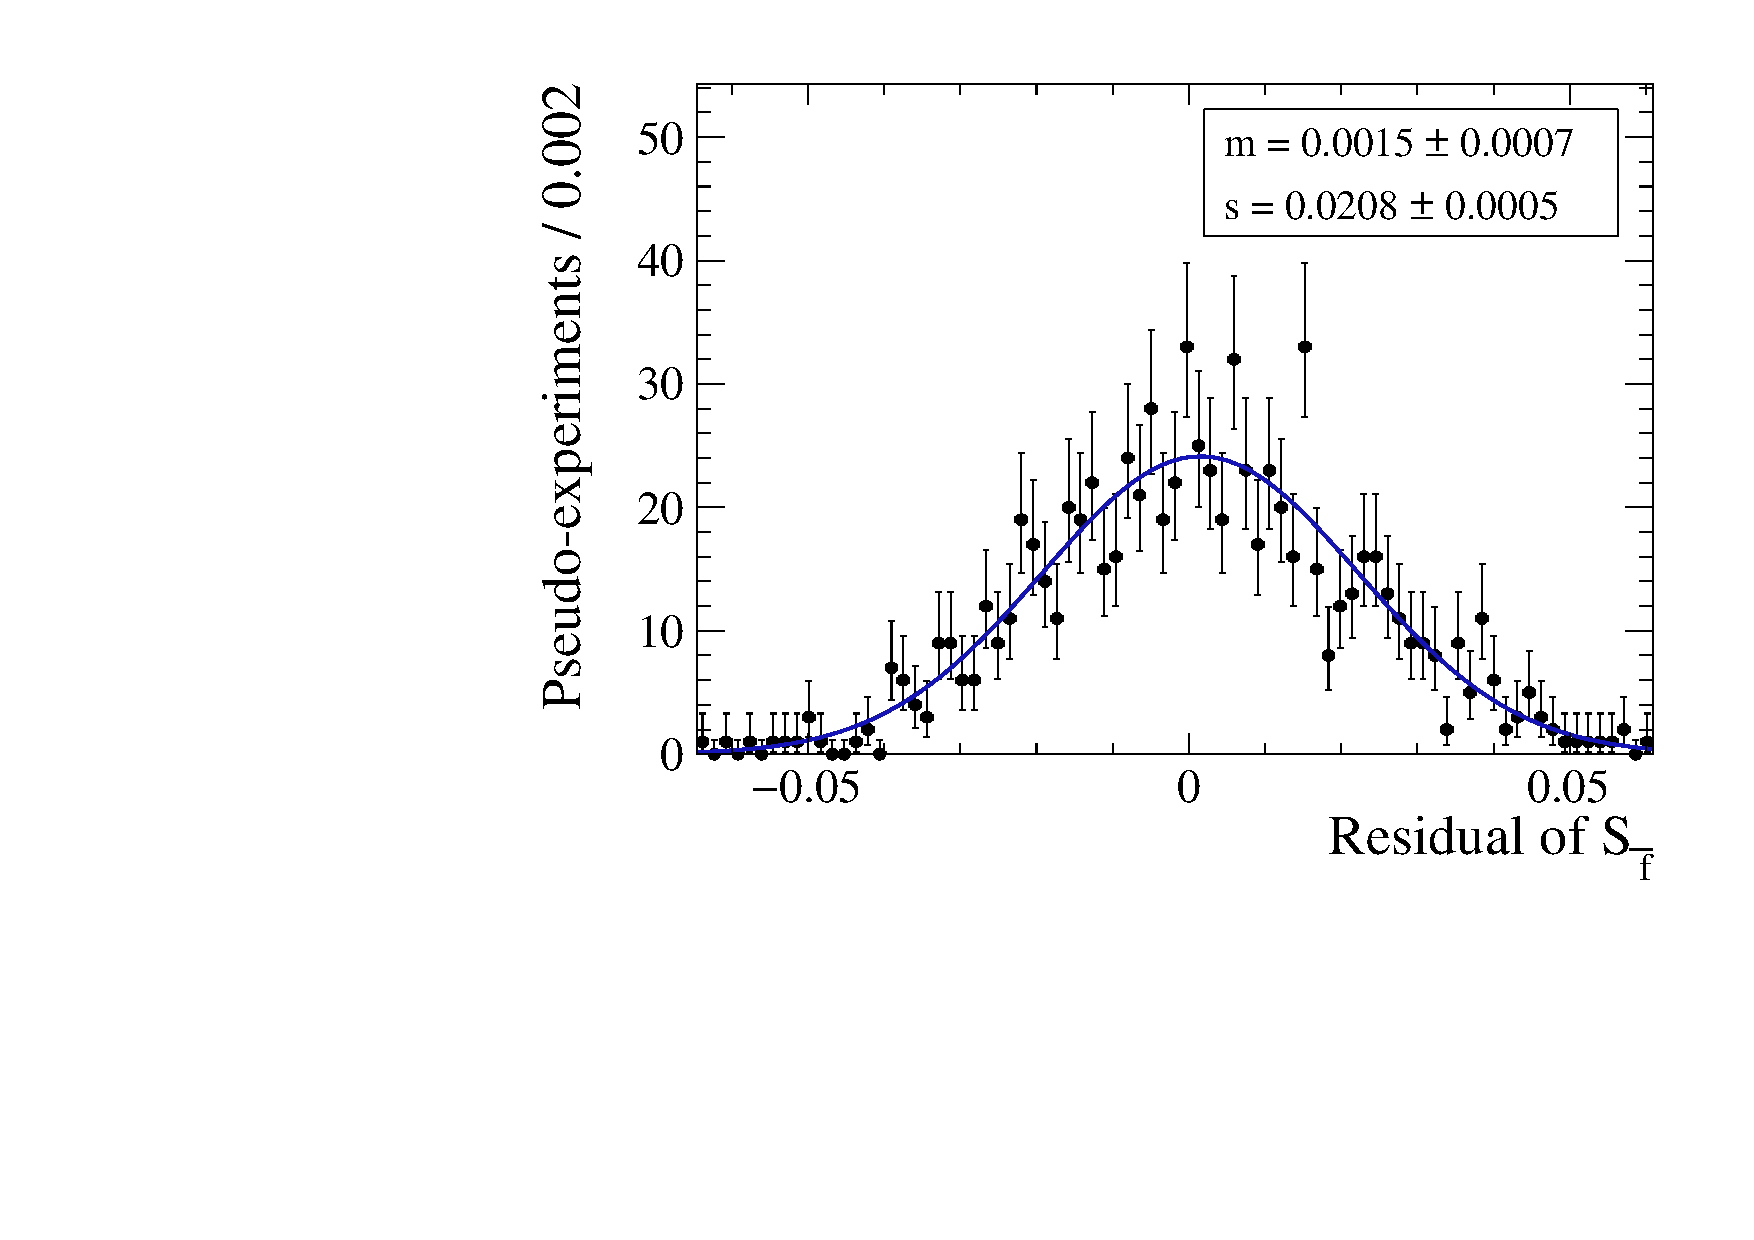
\includegraphics[width=0.4\textwidth]{06Systematics/figs/FT_Sfbar_res.pdf}
	\end{center}
        \vspace{-2mm}
	\caption{Distribution of $S_f$ (left) and $S_{\bar f}$ (right) residuals for the determination of the systematic uncertainty due to the tagging calibration
	models.}
	\label{fig:FTSystToys}
\end{figure}

%-------------------------------------------------------------------------------
\subsubsection{Flavour tagging efficiency asymmetries}
\label{sec:syst_toys_tageffAsym}

Toys are generated with the flavour tagging asymmetries set to their (negative) estimate from simulation minus their
uncertainty, namely \SI{-0.14}{\percent} and \SI{-0.13}{\percent} for the OS and SS tagger, respectively.
The distributions of the residuals of \Sf~and \Sfb~are shown in Fig.~\ref{fig:FTEffAsym}. The residuals are not compatible with
zero and therefore they are assigned as systematic uncertainties.
\begin{figure}[t]
	\begin{center}
		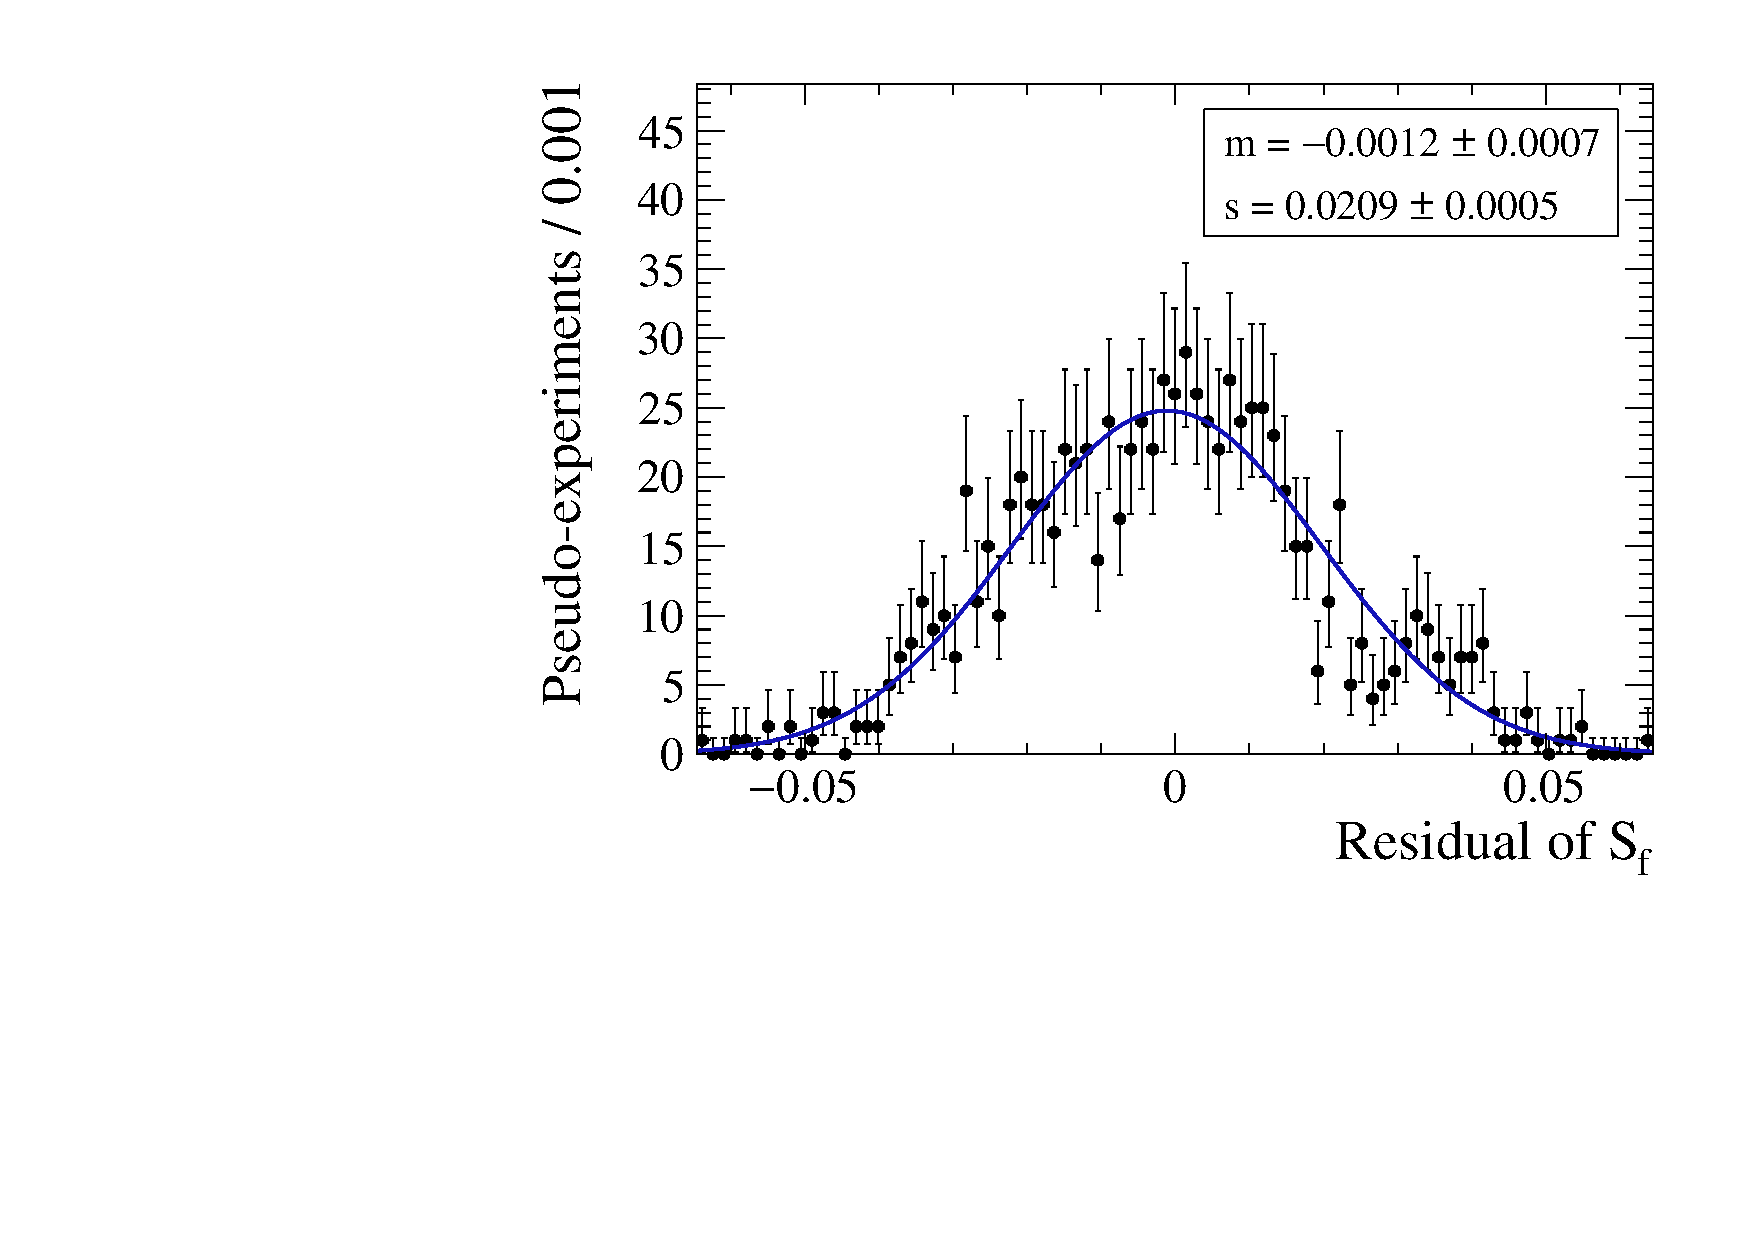
\includegraphics[width=0.4\textwidth]{06Systematics/figs/FTeffAsym_Sf_res.pdf}
		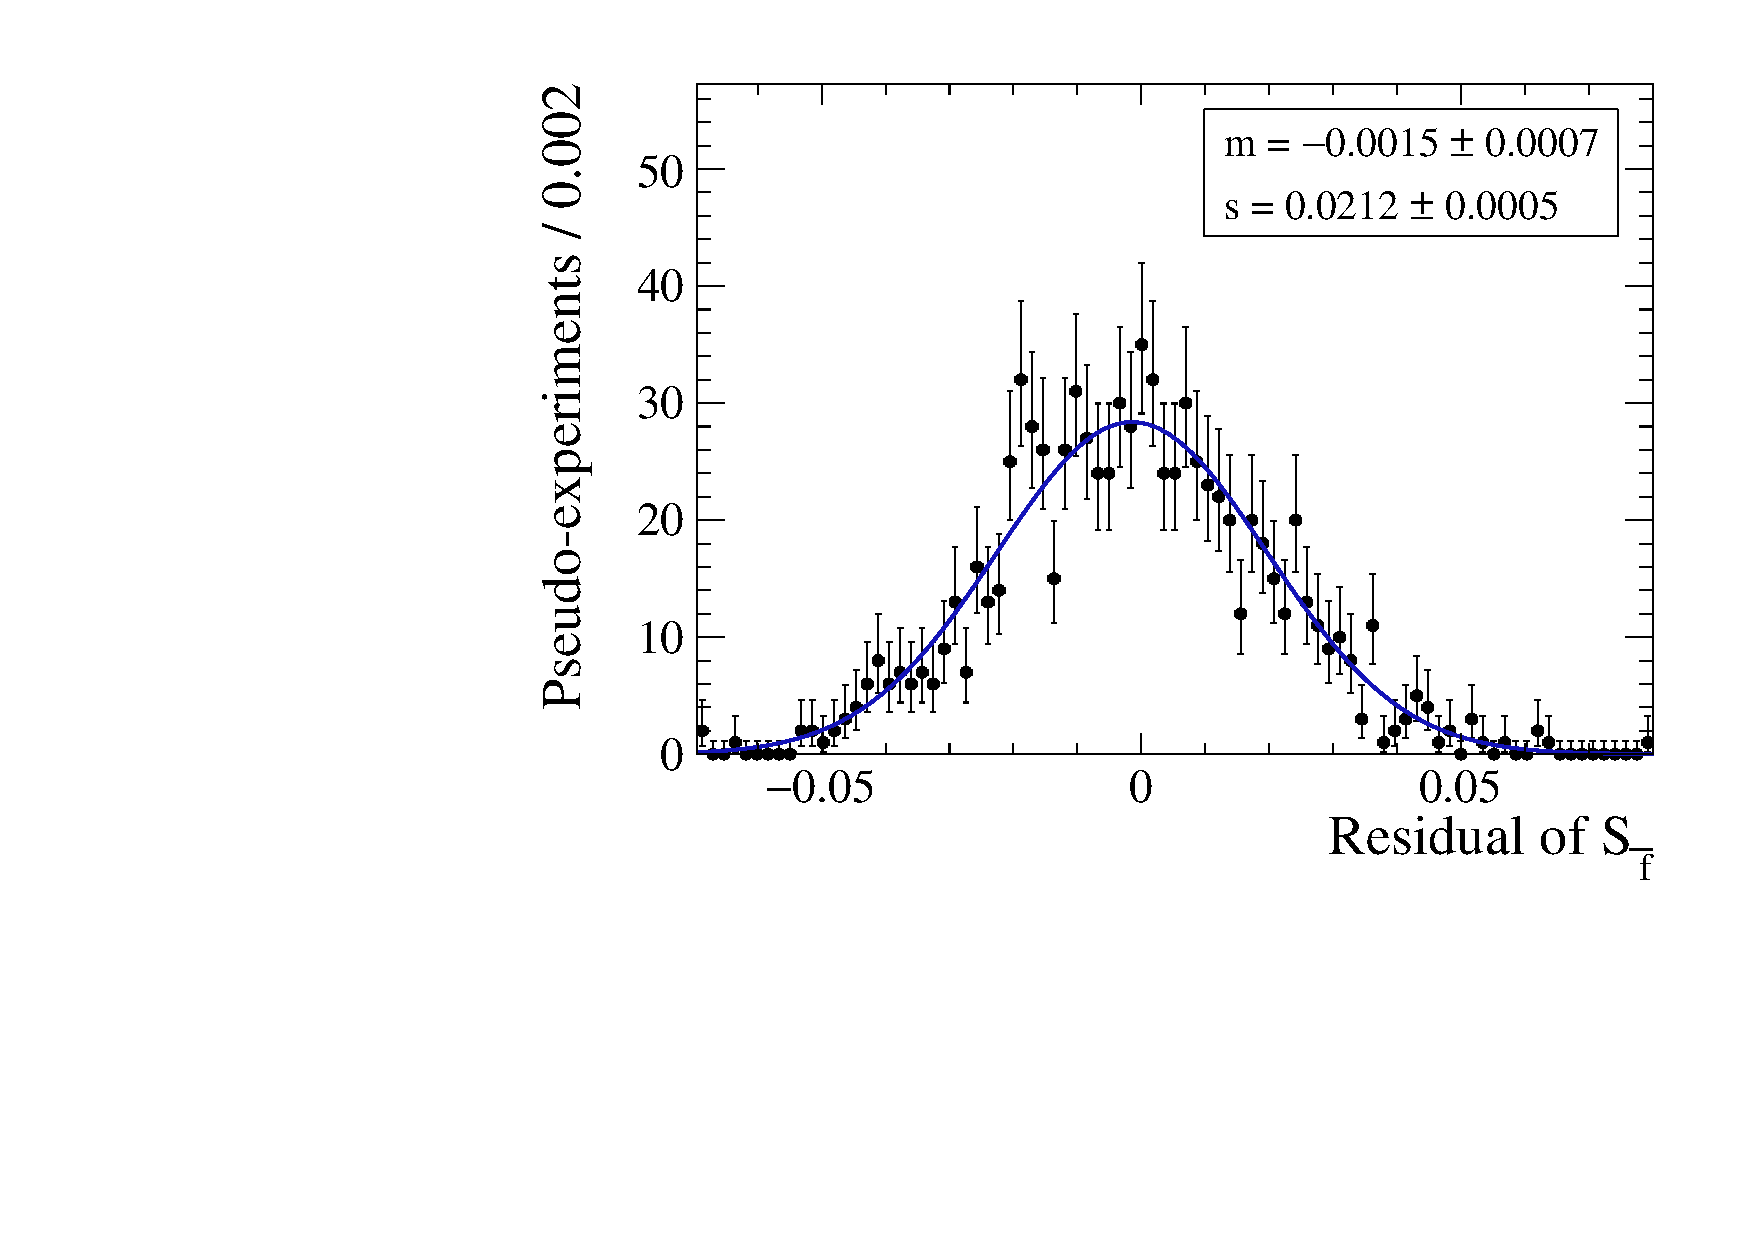
\includegraphics[width=0.4\textwidth]{06Systematics/figs/FTeffAsym_Sfbar_res.pdf}
	\end{center}
        \vspace{-2mm}
	\caption{Distribution of $S_f$ (left) and $S_{\bar f}$ (right) residuals for the determination of the systematic uncertainty due to the assumption on
	the flavour tagging efficiency asymmetry.}
	\label{fig:FTEffAsym}
\end{figure}

%-------------------------------------------------------------------------------
\subsubsection{Acceptance model}
\label{sec:syst_toys_acceptancemodel}

The acceptance model is modified in the generation by replacing the nominal knots for the spline function with new knots,
namely at 0.4, 0.45, 0.8, 1.3, 2.5, 6.0, and 12.0 ps. The distribution of the residuals of
\Sf~and \Sfb~are shown in Fig.~\ref{fig:acceptanceSystToys}. Residuals consistent with zero are found
and therefore the uncertainty on the residuals is assigned as systematic uncertainty.
\begin{figure}[t]
	\begin{center}
		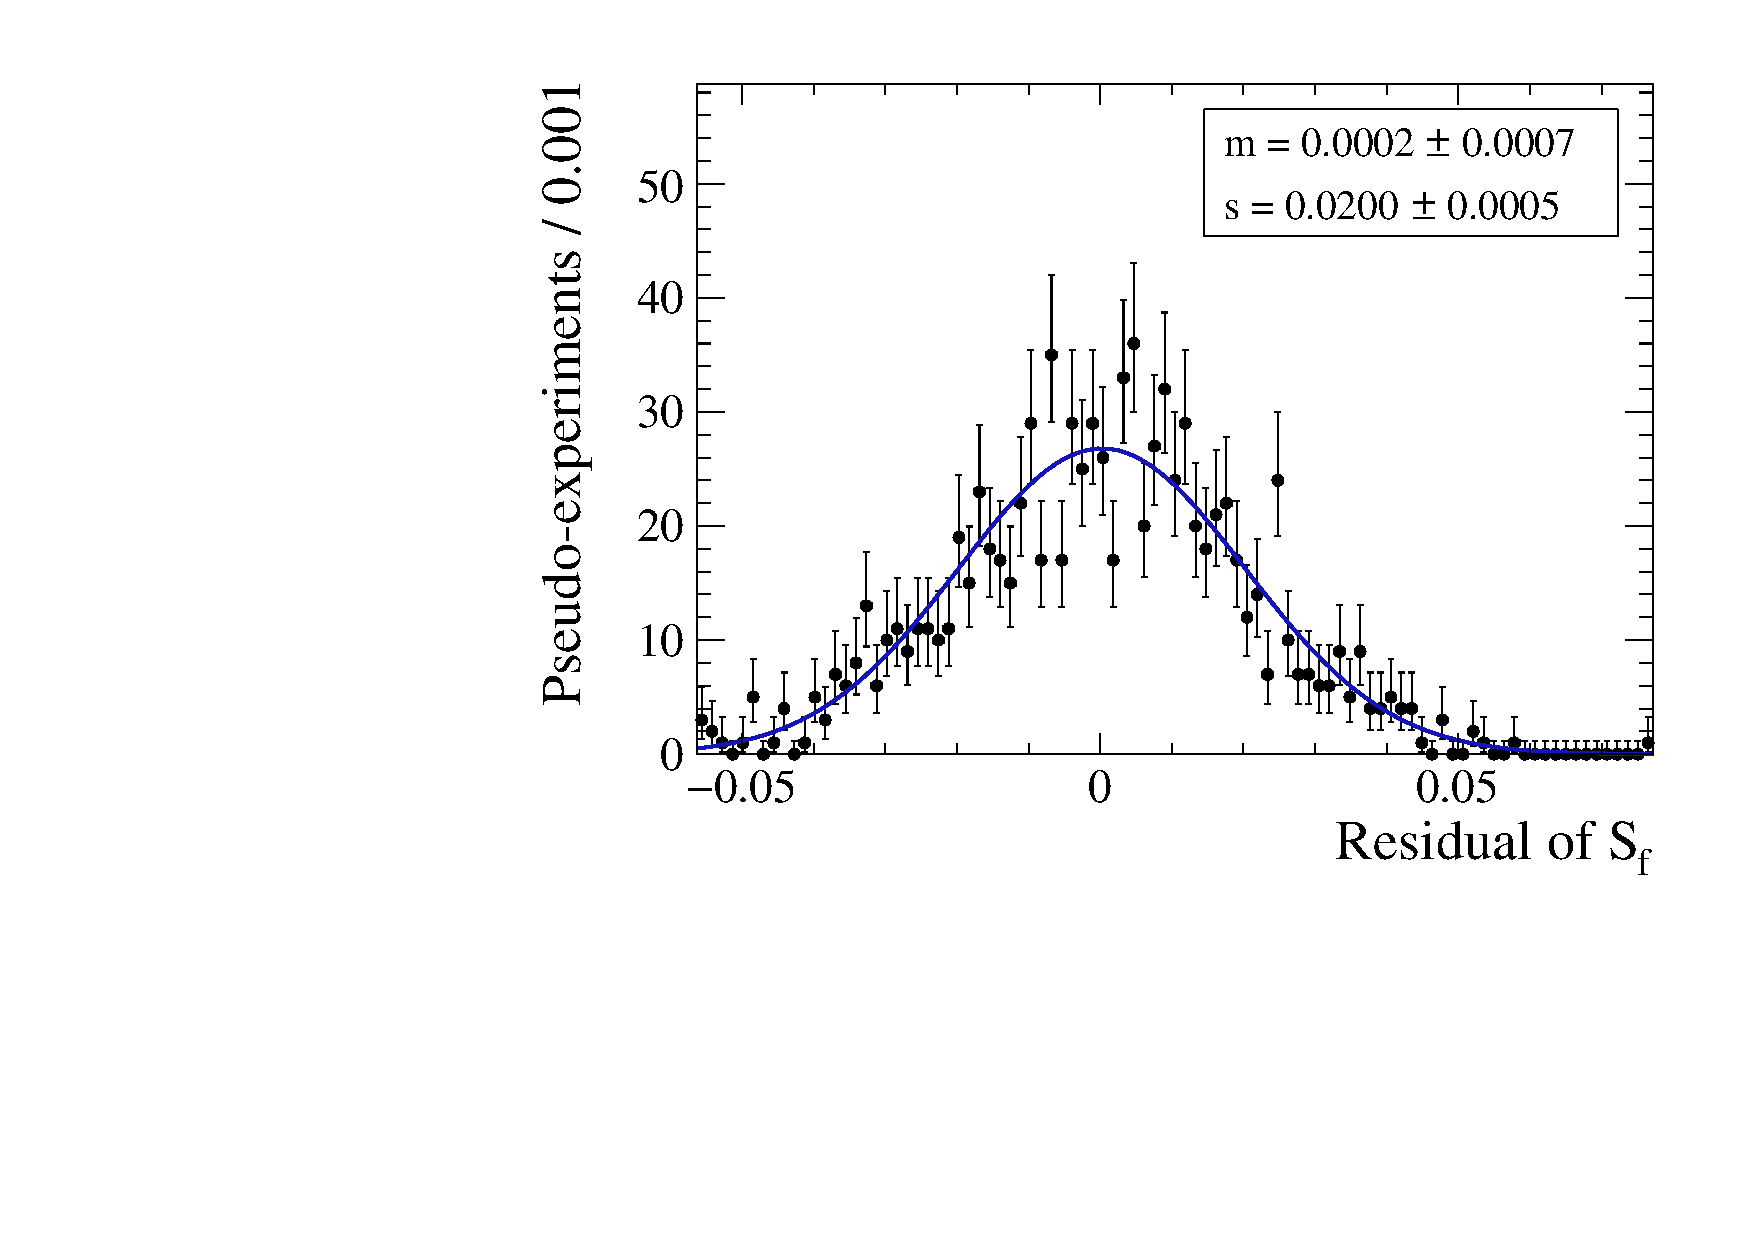
\includegraphics[width=0.4\textwidth]{06Systematics/figs/accept_Sf_res.pdf}
		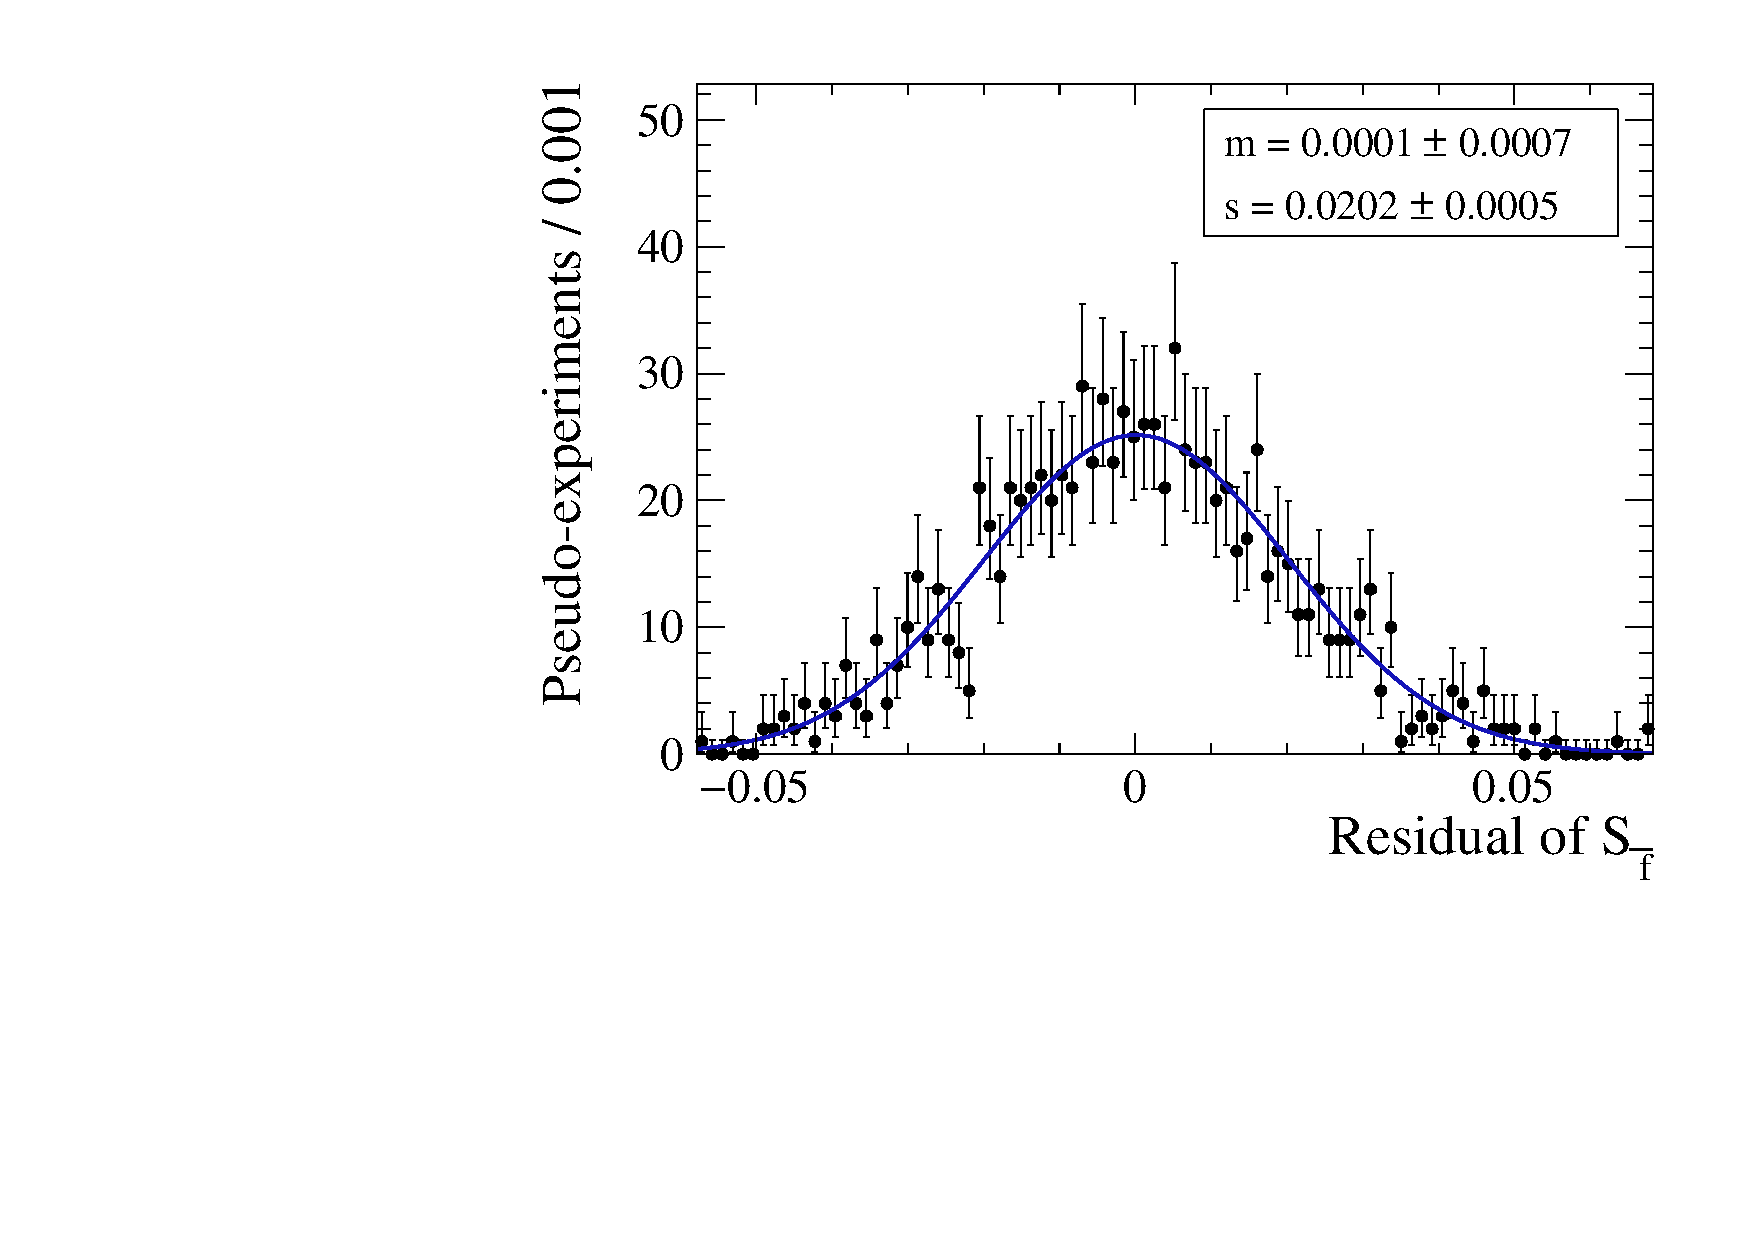
\includegraphics[width=0.4\textwidth]{06Systematics/figs/accept_Sfbar_res.pdf}
	\end{center}
        \vspace{-2mm}
	\caption{Distribution of $S_f$ (left) and $S_{\bar f}$ (right) residuals for the determination of the systematic uncertainty due to the acceptance model.}
	\label{fig:acceptanceSystToys}
\end{figure}

\subsubsection{Decay time resolution}
\label{sec:syst_toys_resolution}
Toys are generated with time resolutions $20\fs$ larger and $20\fs$ smaller than the nominal value of 55\fs.
The distributions of the fitted value of \Sf~and \Sfb~are shown in Fig.~\ref{fig:ToysAllFixedCPloRes}.
The largest residual is considered as overall systematic uncertainty.
\begin{figure}[t]
        \begin{center}
                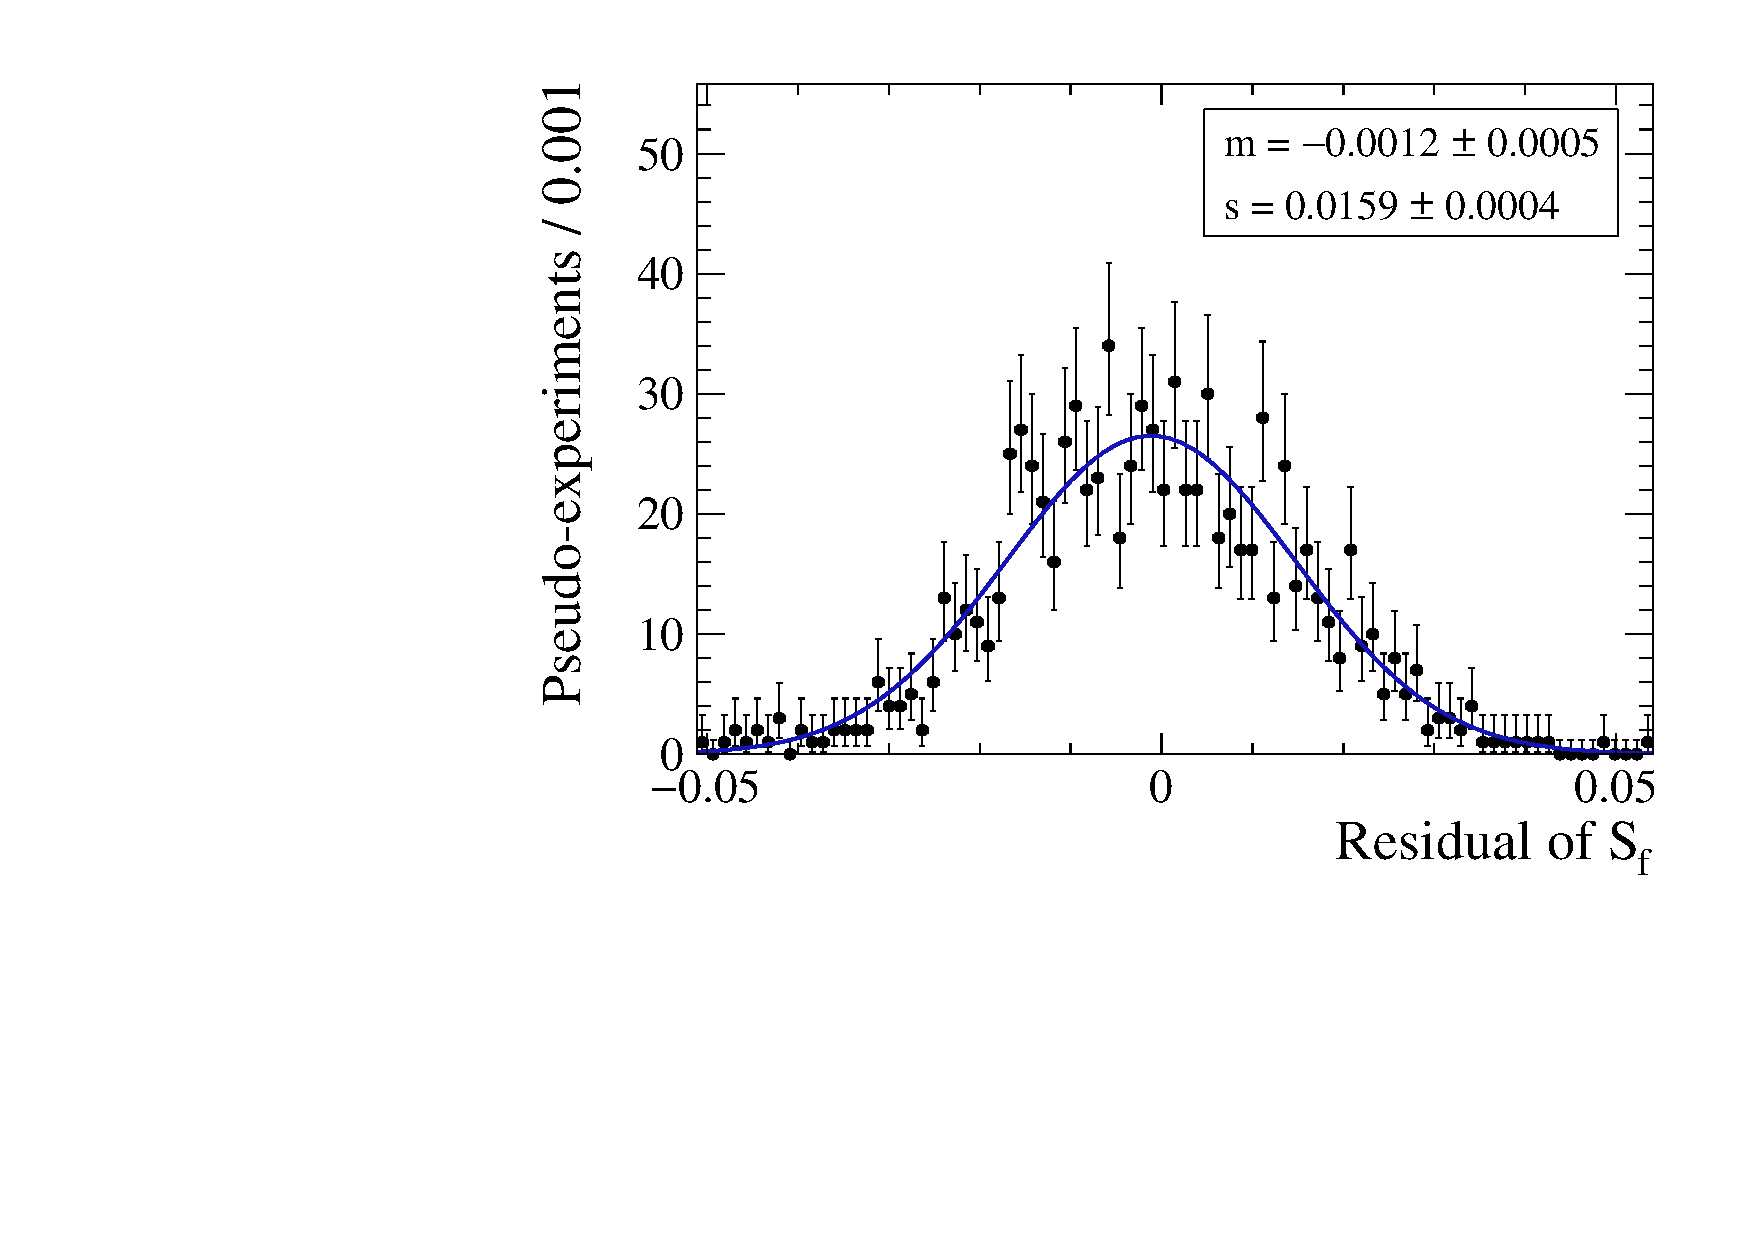
\includegraphics[width=0.4\linewidth]{06Systematics/figs/ResHigh_Sf_res.pdf}
                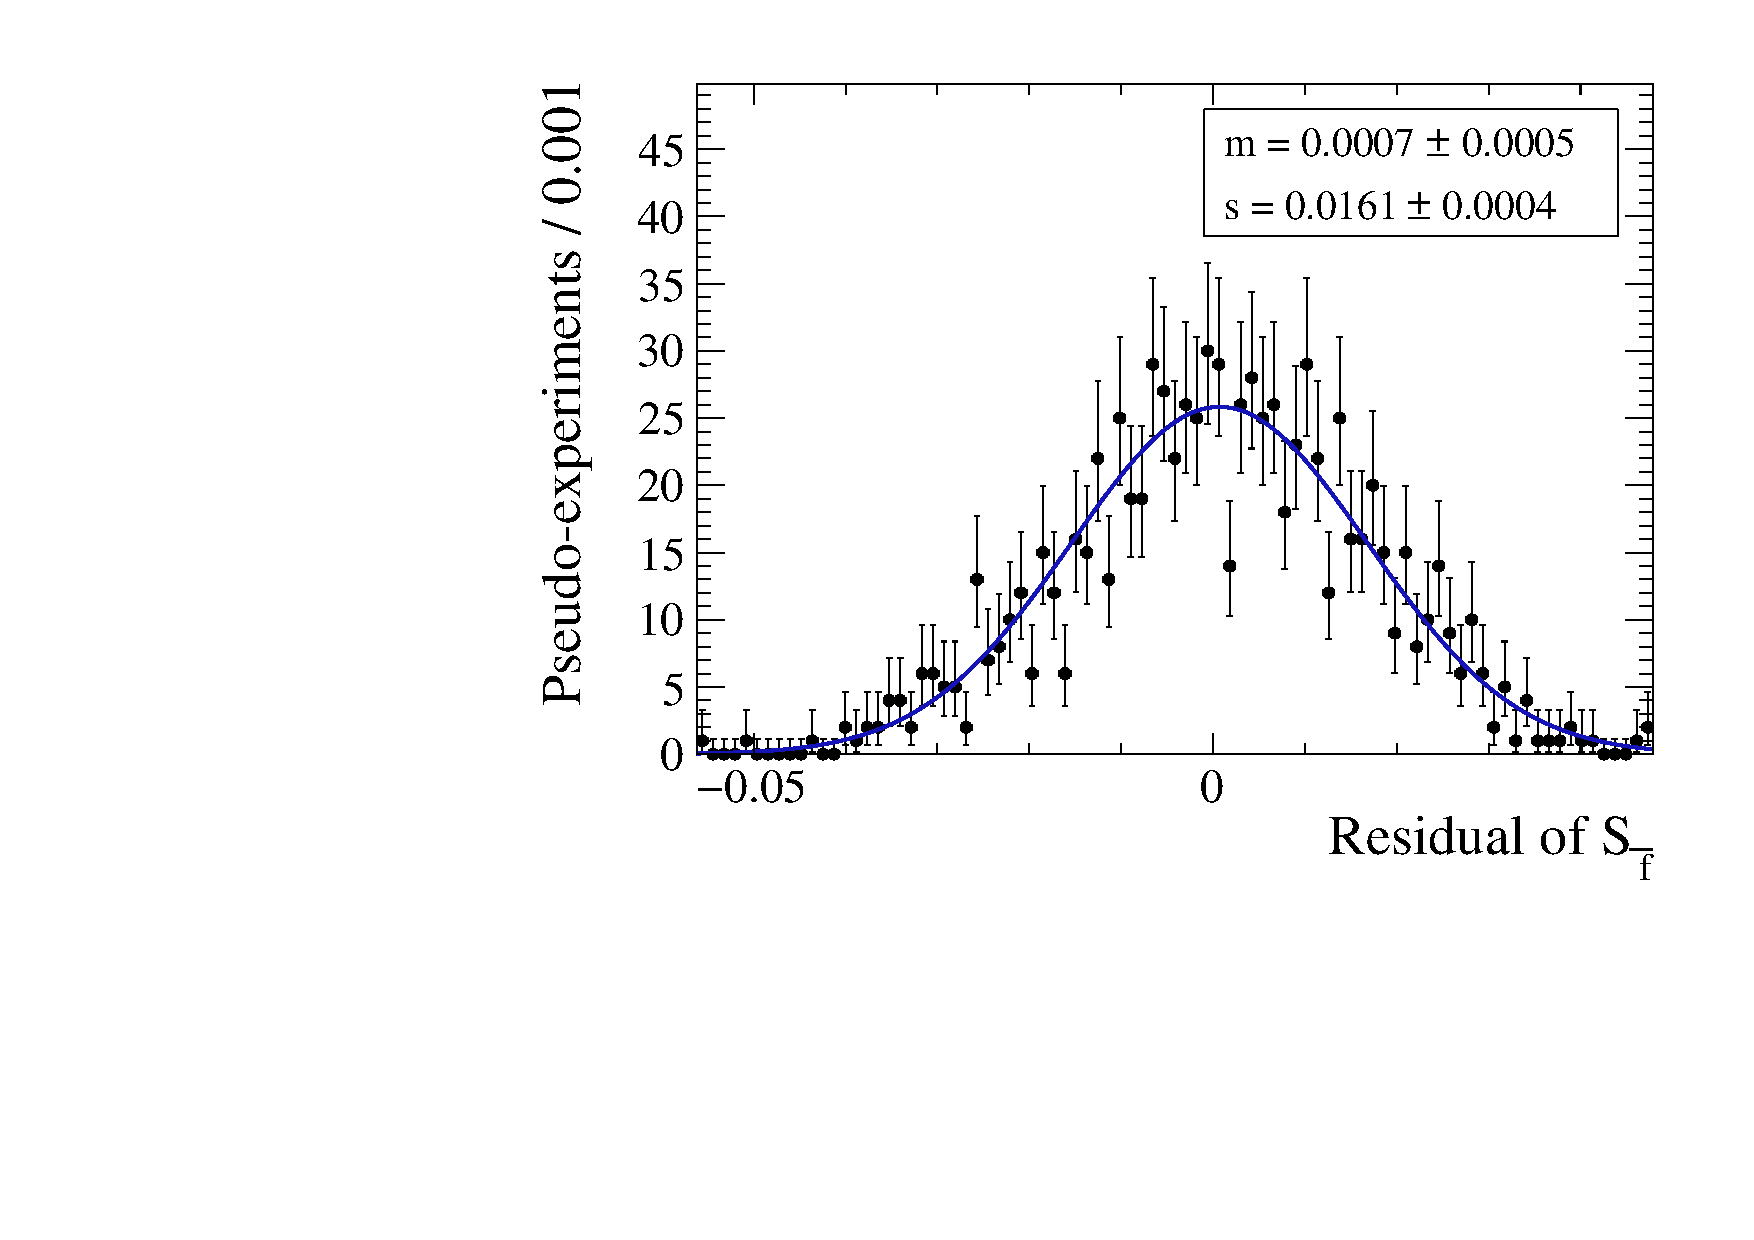
\includegraphics[width=0.4\linewidth]{06Systematics/figs/ResHigh_Sfbar_res.pdf} \\
                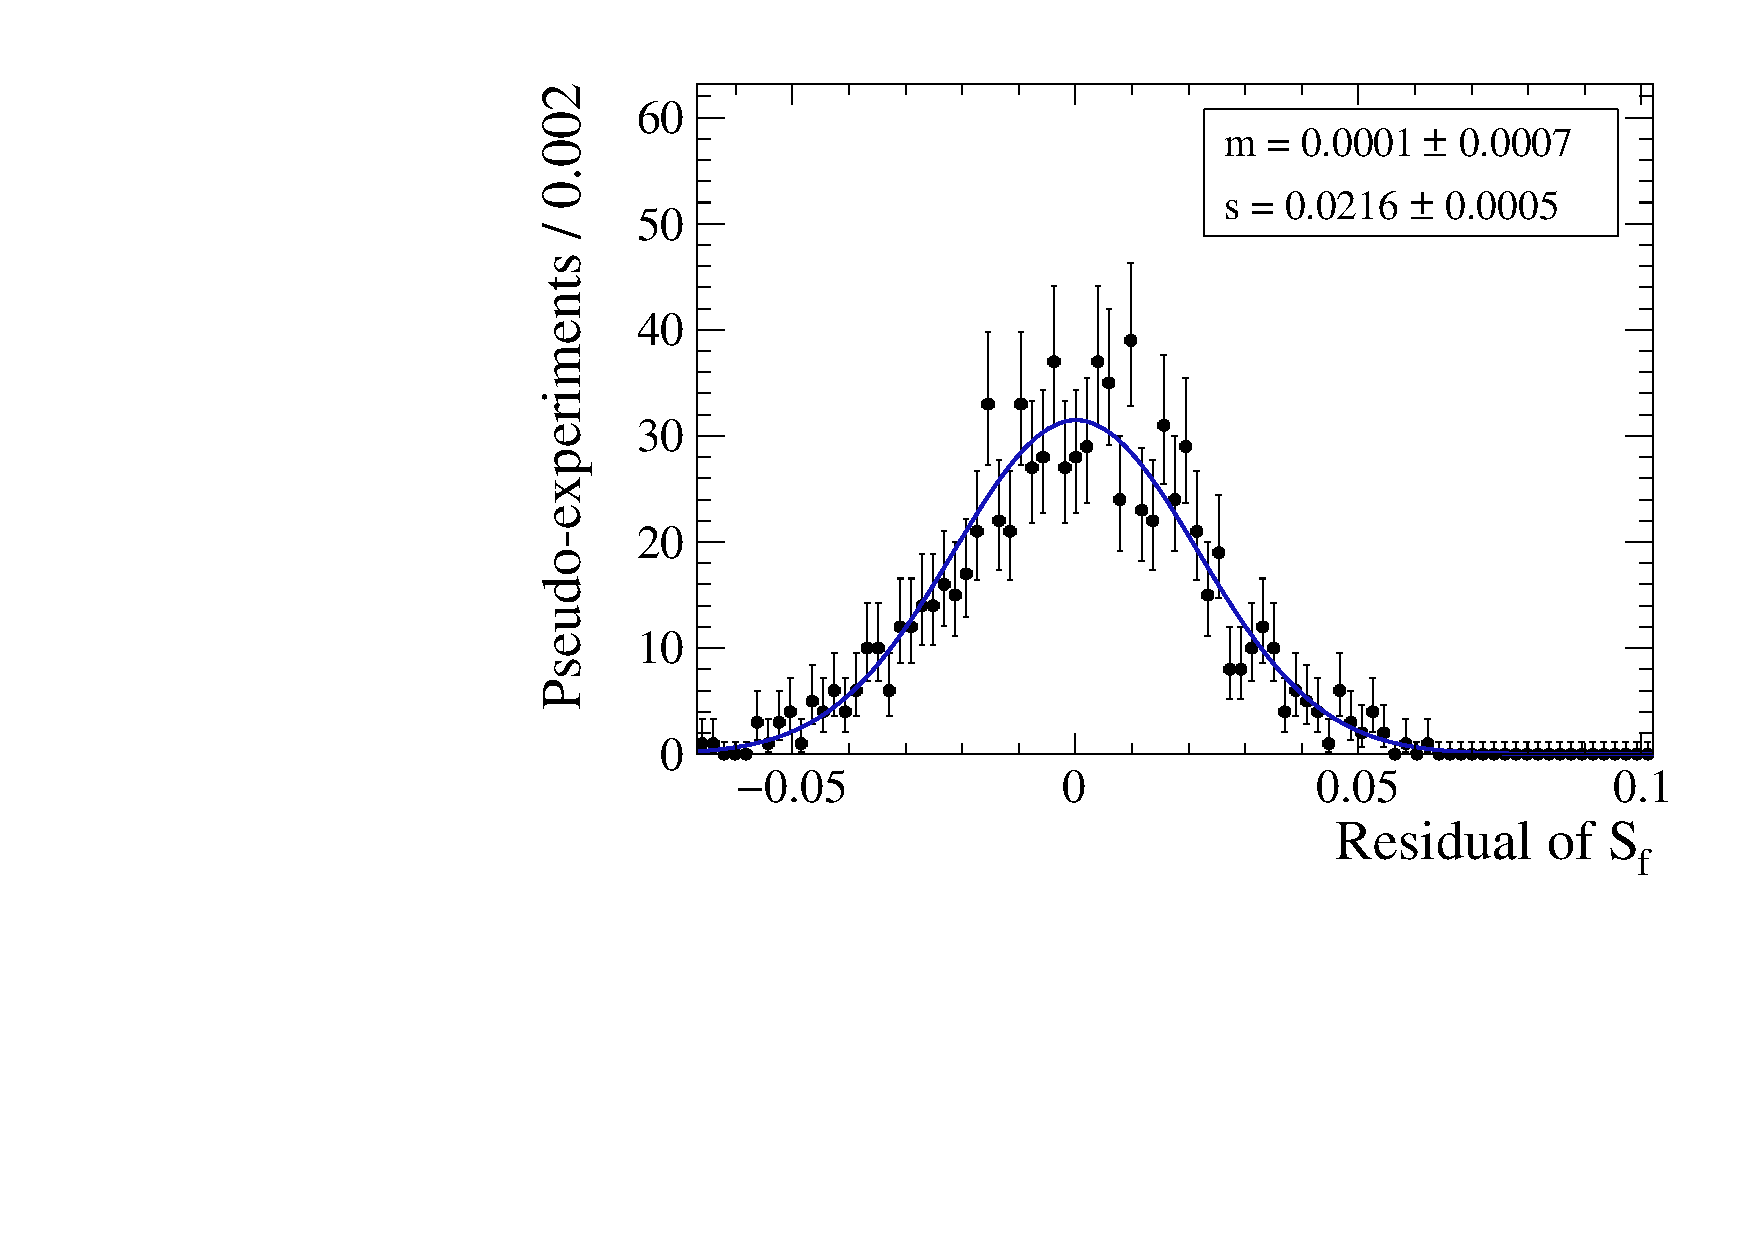
\includegraphics[width=0.4\linewidth]{06Systematics/figs/ResLow_Sf_res.pdf}
                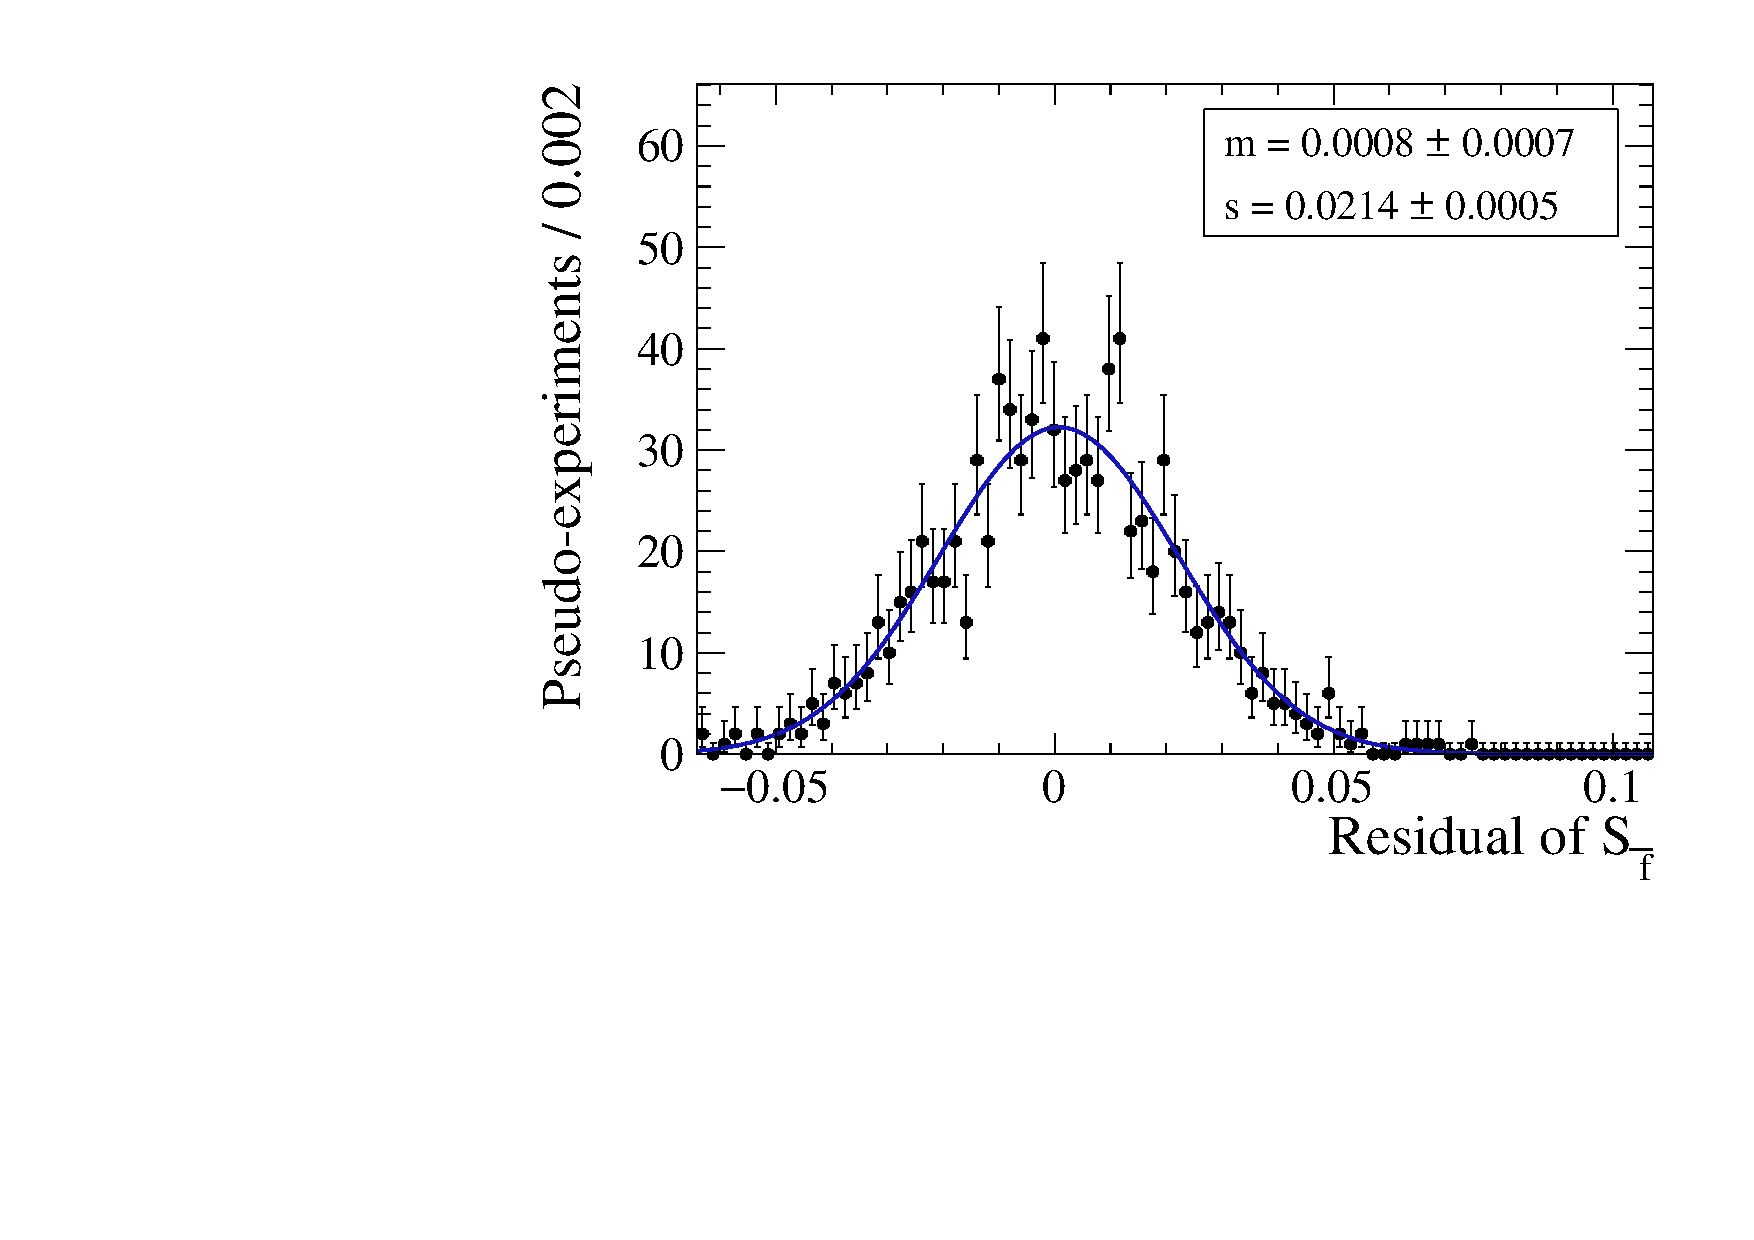
\includegraphics[width=0.4\linewidth]{06Systematics/figs/ResLow_Sfbar_res.pdf}
                \end{center}
        \vspace{-2mm}
        \caption{Distribution of $S_f$ (left) and $S_{\bar f}$ (right) residuals for the determination of the systematic uncertainty due
        to the resolution model. Top: \SI{75}{\fs} resolution model. Bottom: \SI{35}{\fs} resolution
        model. }
        \label{fig:ToysAllFixedCPloRes}
\end{figure}

%-------------------------------------------------------------------------------
\subsubsection[Fixed $C_f$]{Fixed \boldmath{$C_f$}}
\label{sec:syst_toys_fixC}

Toys are generated with $C_f=-C_{\bar f}$ set to the average of the measurements by \belle~and \babar~minus the
largest uncertainty among the two measurements, namely $0.993$~\cite{Aubert:2008zi, Das:2010be}.
The distributions of the residuals of \Sf~and \Sfb~are shown in Fig.~\ref{fig:CSystToys}. Residuals
consistent with zero are found, therefore the uncertainty on the residuals is assigned as systematic
uncertainty.
\begin{figure}[htbp]
	\begin{center}
		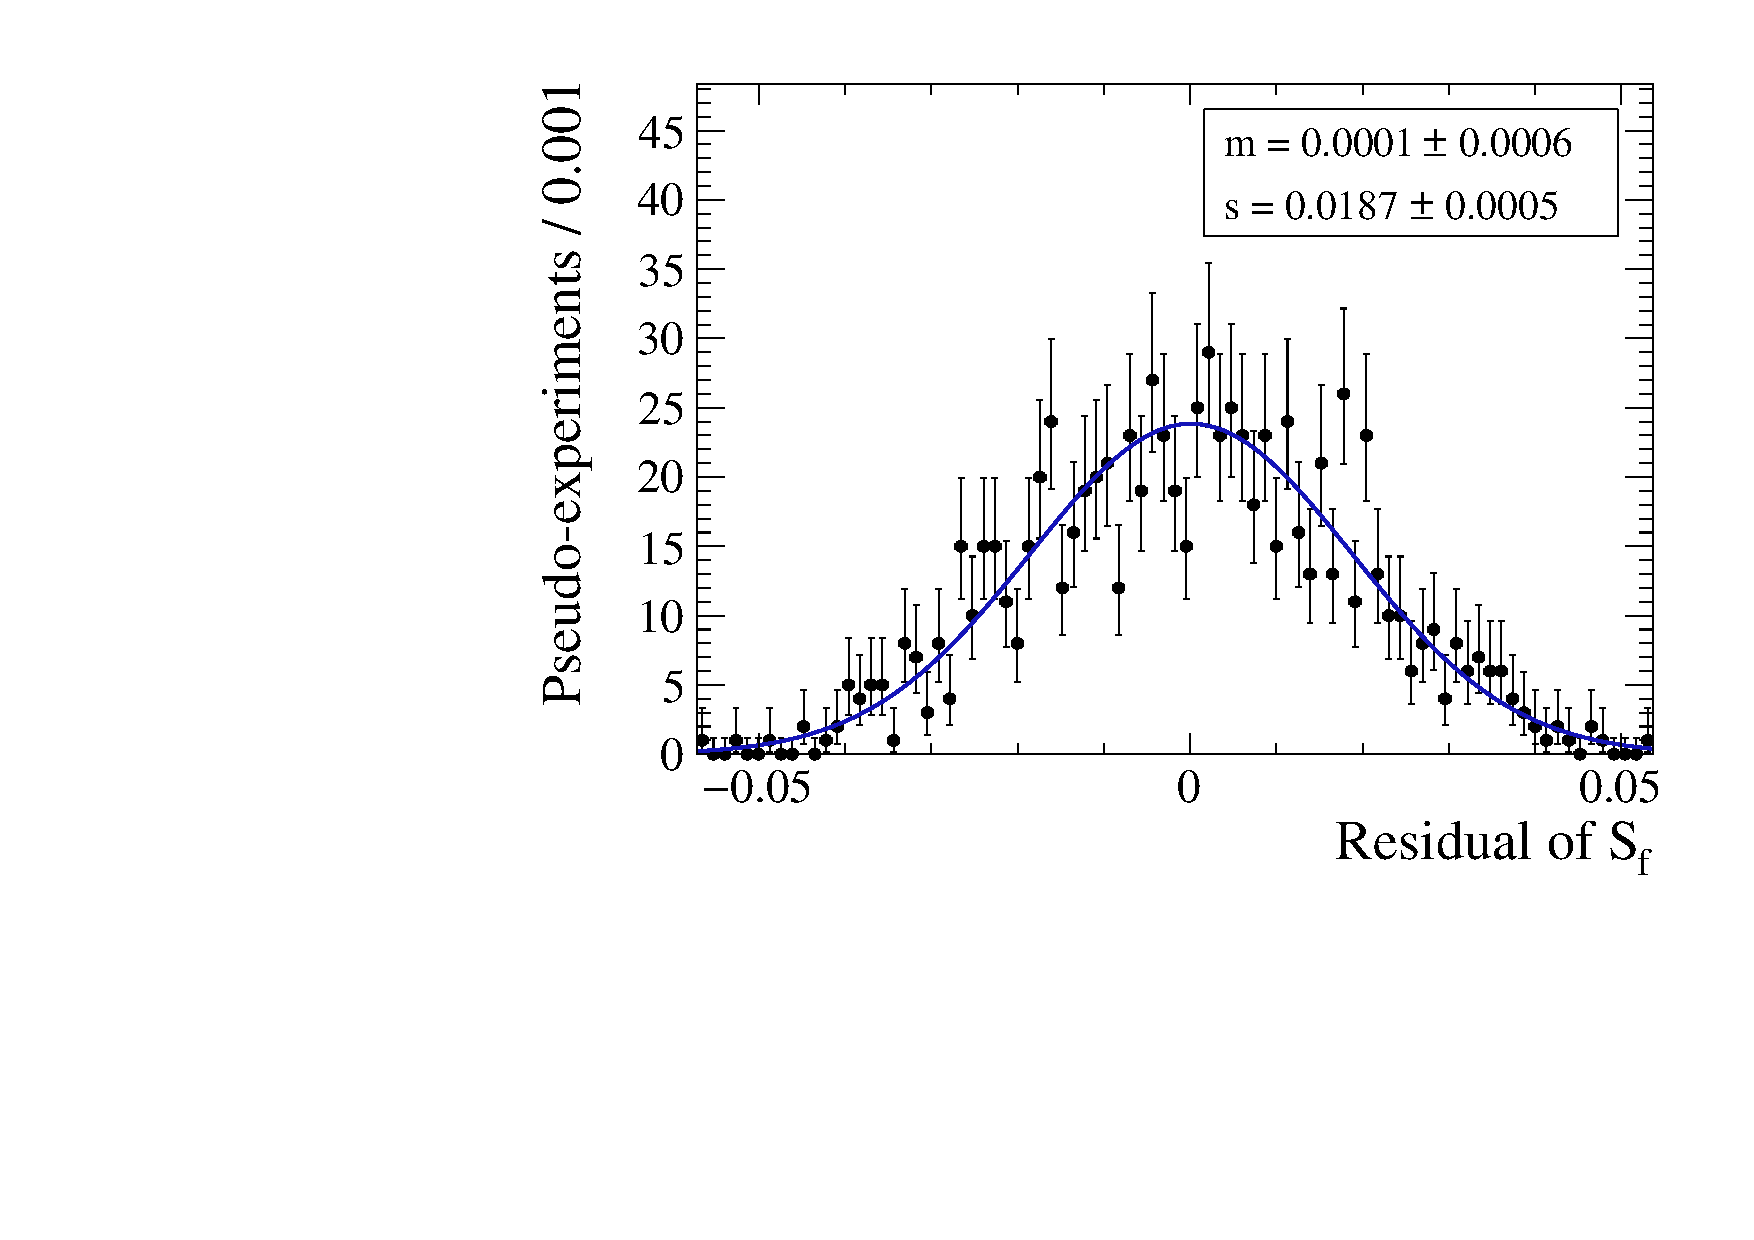
\includegraphics[width=0.4\textwidth]{06Systematics/figs/C_Sf_res.pdf}
		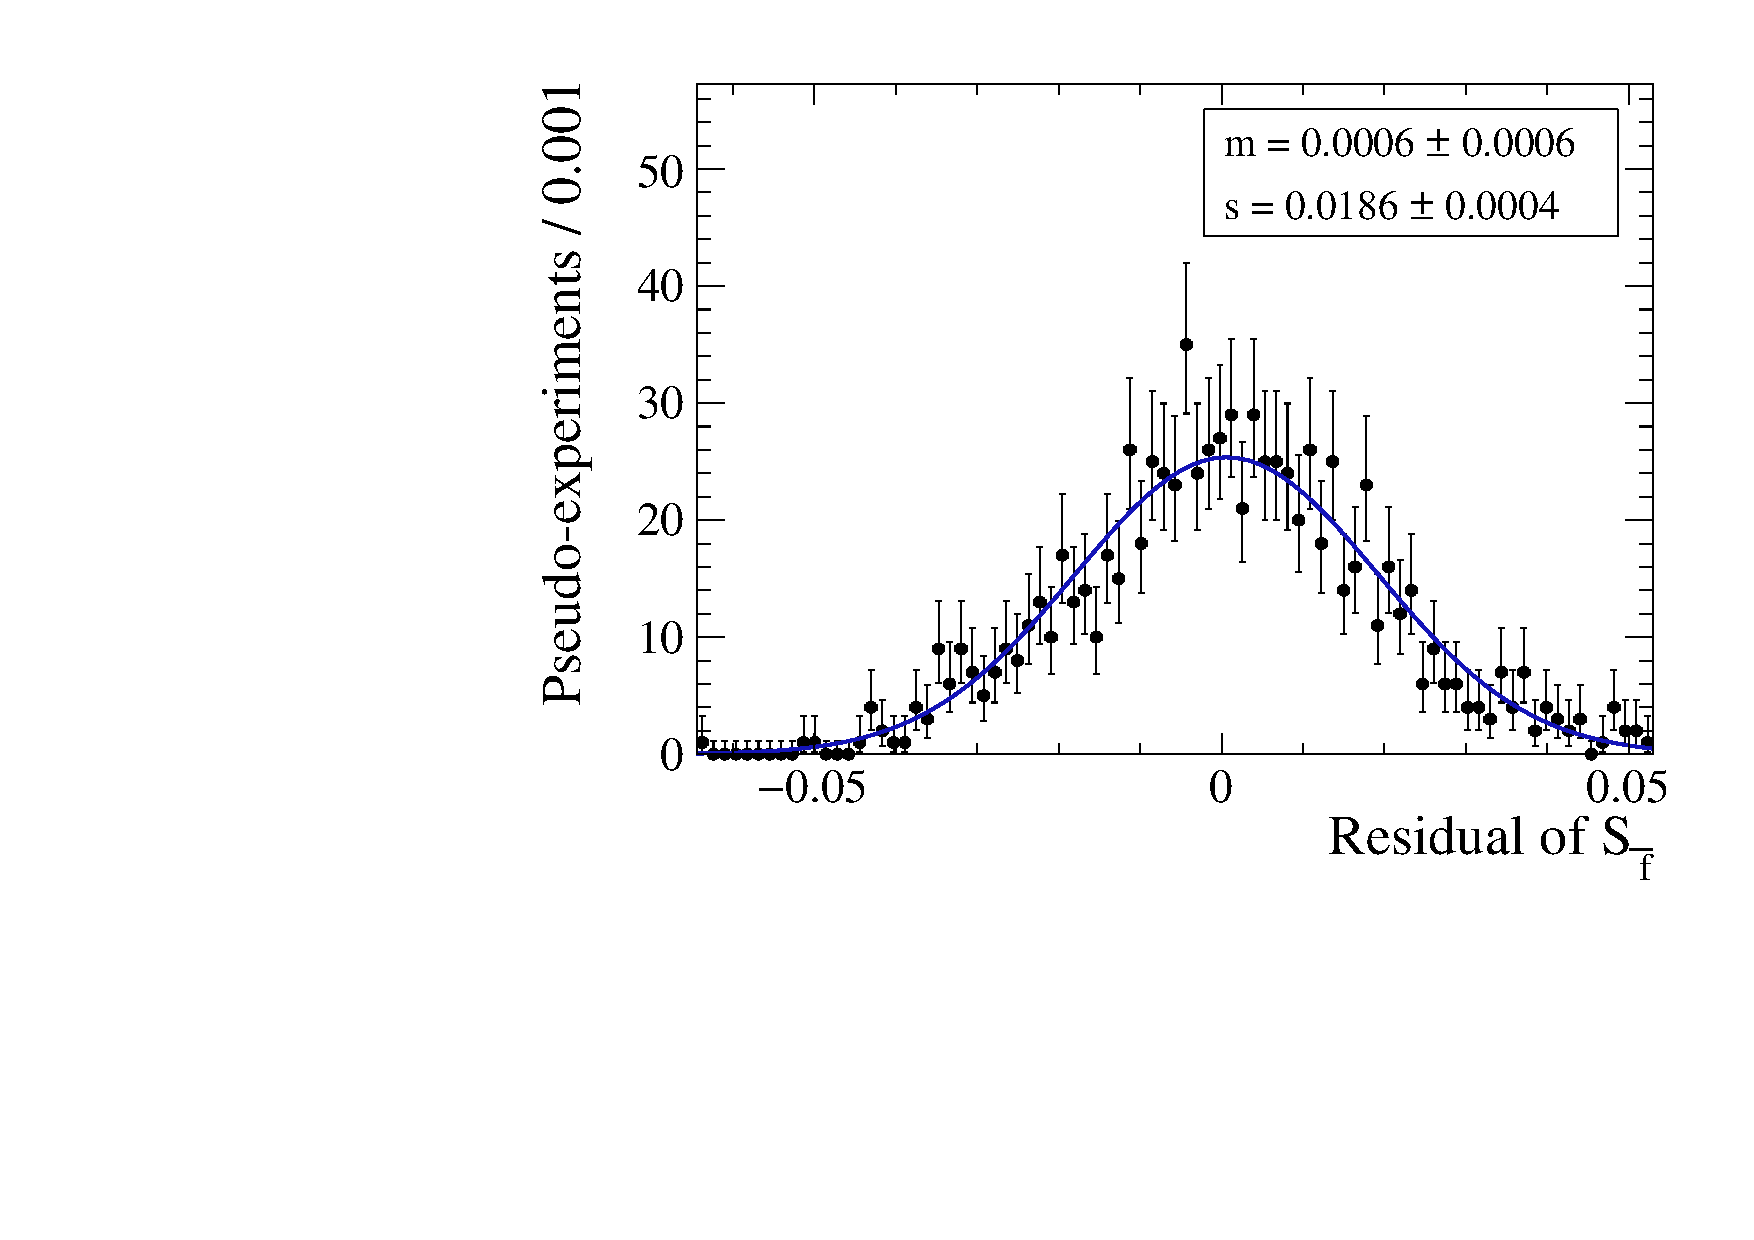
\includegraphics[width=0.4\textwidth]{06Systematics/figs/C_Sfbar_res.pdf}
	\end{center}
        \vspace{-2mm}
	\caption{Distribution of $S_f$ (left) and $S_{\bar f}$ (right) residuals for the determination of the systematic uncertainty due to the assumption $C_f=-C_{\bar f}=1$.}
	\label{fig:CSystToys}
\end{figure}

%-------------------------------------------------------------------------------
\subsubsection[Fixed $\Delta\Gamma$]{Fixed \boldmath{$\Delta\Gamma$}}
\label{sec:syst_toys_deltaGamma}

Toys are generated with \DG~set to the world average value plus its uncertainty, namely $0.0079\ps^{-1}$~\cite{HFAG}.
Moreover, the $D_{f}$ and $D_{\bar f}$ coefficients (defined in Eqs.~\ref{eq:P0tof}-\ref{eq:P0bartofbar}) have been fixed to their expected values of $-0.0103$ and $-0.0155$,
the same used in the Monte Carlo production of the $\Bz\to \Dm\pip$ sample (Appendix~\ref{app:mcgen}). The distribution of the residuals of \Sf~and
\Sfb~are shown in Fig.~\ref{fig:DGSystToys}. Residuals consistent with zero are found, therefore the uncertainty
on the residuals is assigned as systematic uncertainty.
\begin{figure}[t]
	\begin{center}
		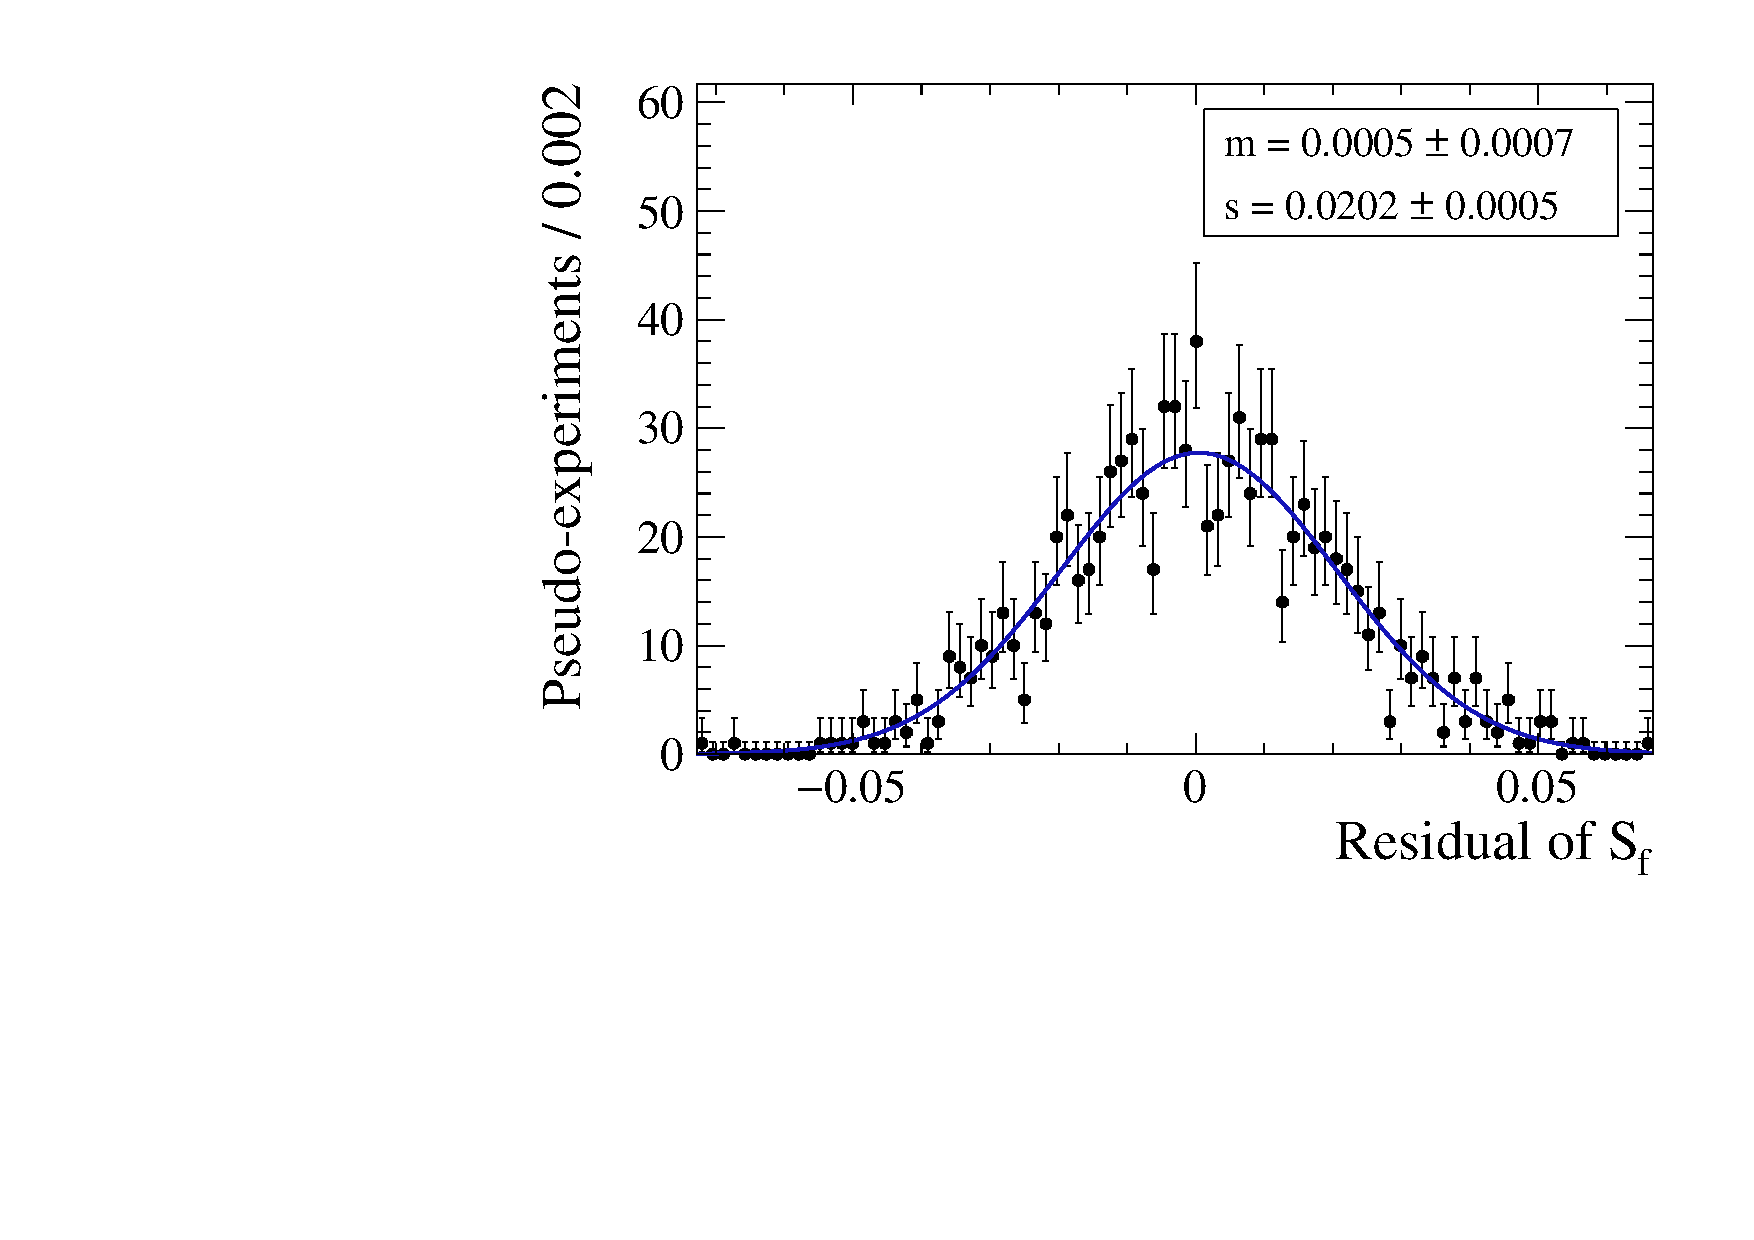
\includegraphics[width=0.4\textwidth]{06Systematics/figs/DG_Sf_res.pdf}
		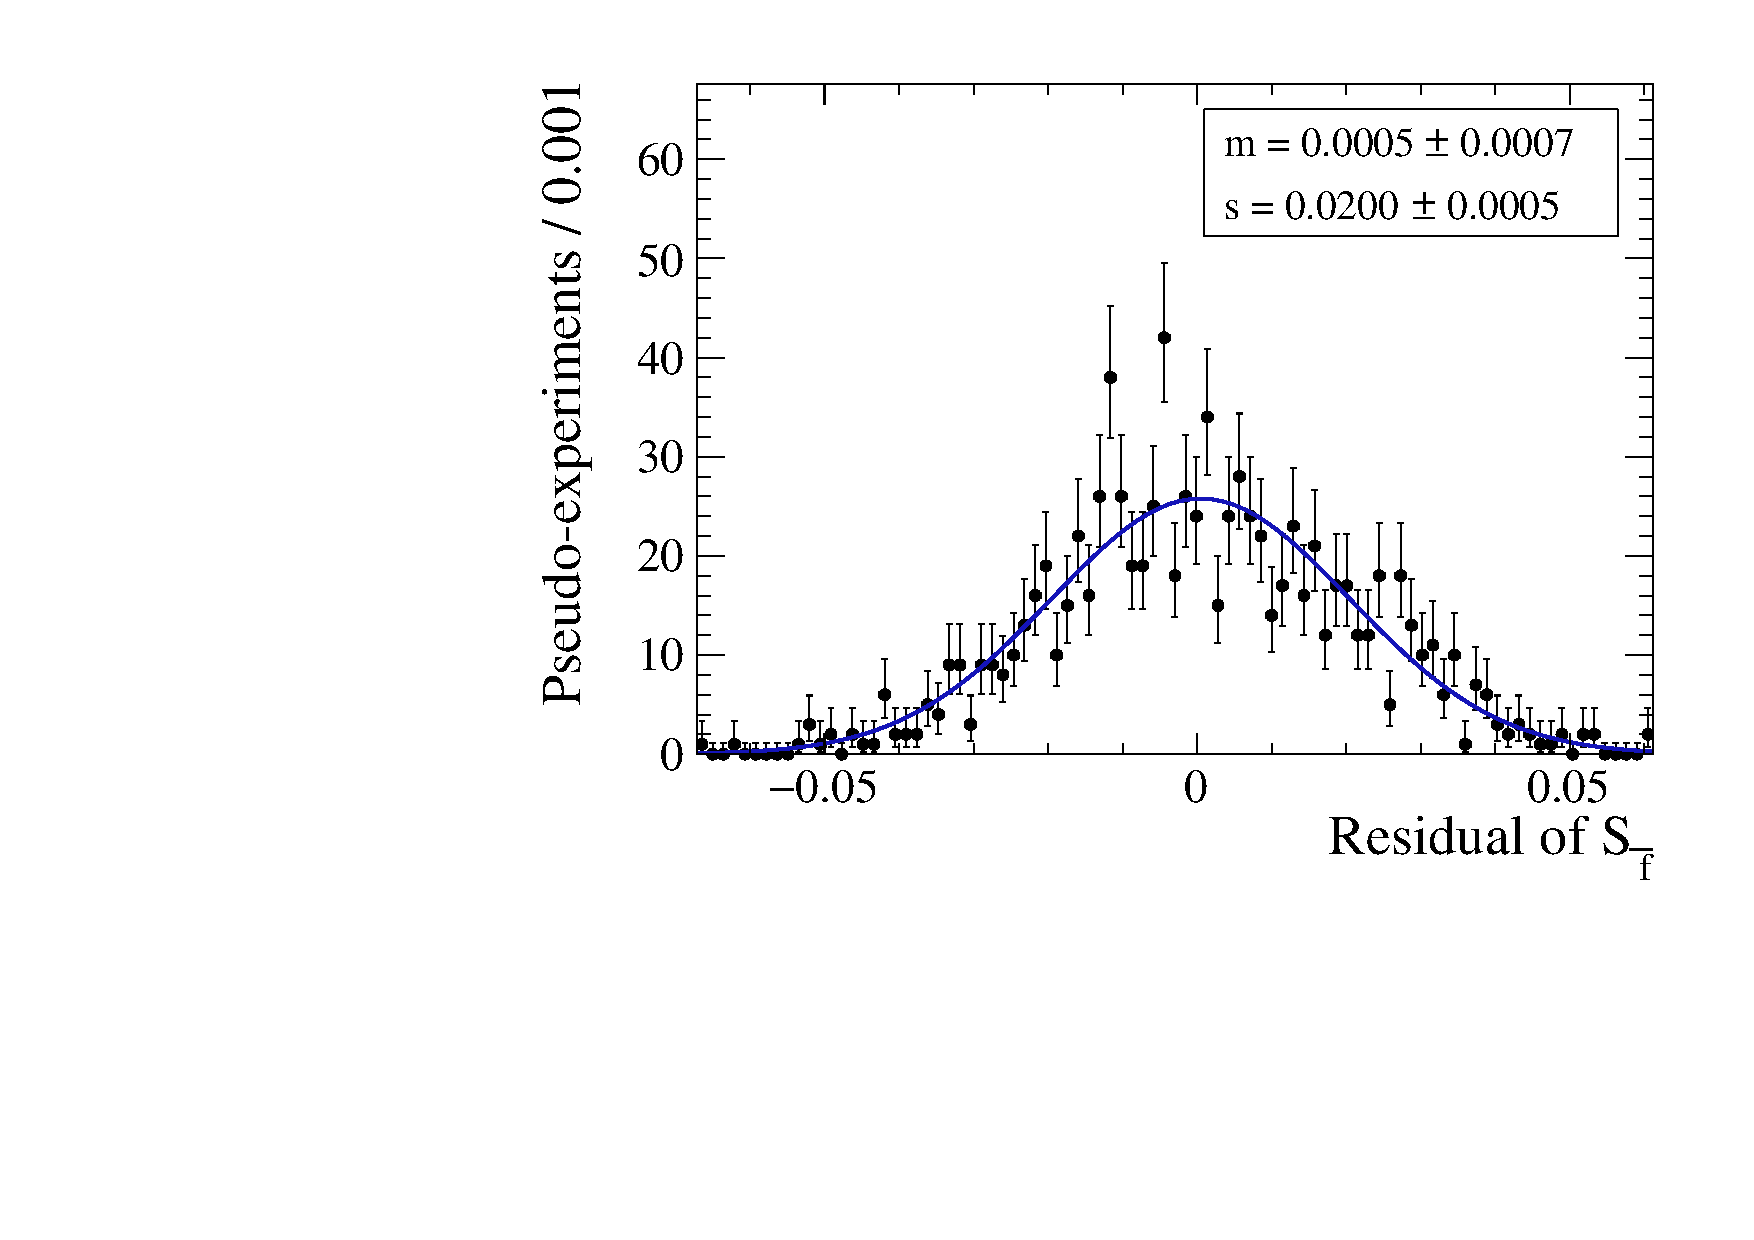
\includegraphics[width=0.4\textwidth]{06Systematics/figs/DG_Sfbar_res.pdf}
	\end{center}
        \vspace{-2mm}
	\caption{Distribution of $S_f$ (left) and $S_{\bar f}$ (right) residuals for the determination of the systematic uncertainty due the assumption $\DG=0$.}
	\label{fig:DGSystToys}
\end{figure}

%!TEX root = ../my_thesis.tex
\subsection{Systematics related to the background subtraction}
\label{sec:syst_mass}
Systematic uncertainties can arise from the choice of the mass fit strategy adopted to calculate \emph{sWeights} (Sec.~\ref{sec:massfit}).
Fit B, used to compute the \emph{sWeights}, is repeated in the full mass window ($[5090,6000]\mevcc$) instead of the narrow signal region ($[5220,5600]\mevcc$).
In this way, the resulting sample is enriched in background events.
The aim of this test is to estimate how much background events (with negative \emph{sWeights}) affect the result for $S_f$ and $S_{\bar f}$ in the final decay time fit.
The fitted total background yield in this new mass fit configuration is $199\,767\pm481$, compared to $34\,102\pm299$ in the nominal fit configuration (Table~\ref{tab:FitBfloating}).
The projection of the PDF used for Fit B in the wide mass range is shown in Fig.~\ref{fig:FitBWideMass}. The new \emph{sWeights} 
are then used in a decay time fit performed on the full sample following the same strategy as reported in Sec.~\ref{sec:datafit}. The correlated disagreement, defined as the difference between the fit results divided by the difference in quadrature between the fitted uncertainties, between the result of this fit and that of the nominal fit is $2.3~\sigma$ for $S_f$ and 
and $1.8~\sigma$ for $S_{\bar f}$. 
Because of this discrepancy, the difference between the newly obtained $S_f$ and $S_{\bar f}$ coefficients and the nominal values is taken as systematic uncertainty, yielding $0.0042$ and $0.0023$ for $S_f$ and $S_{\bar f}$ respectively. The correlation between the systematic uncertainties on $S_f$ and $S_{\bar f}$ is estimated to be $0.7$, as shown in Appendix~\ref{app:corrSyst}.

\begin{figure}[t]
        \begin{center}
                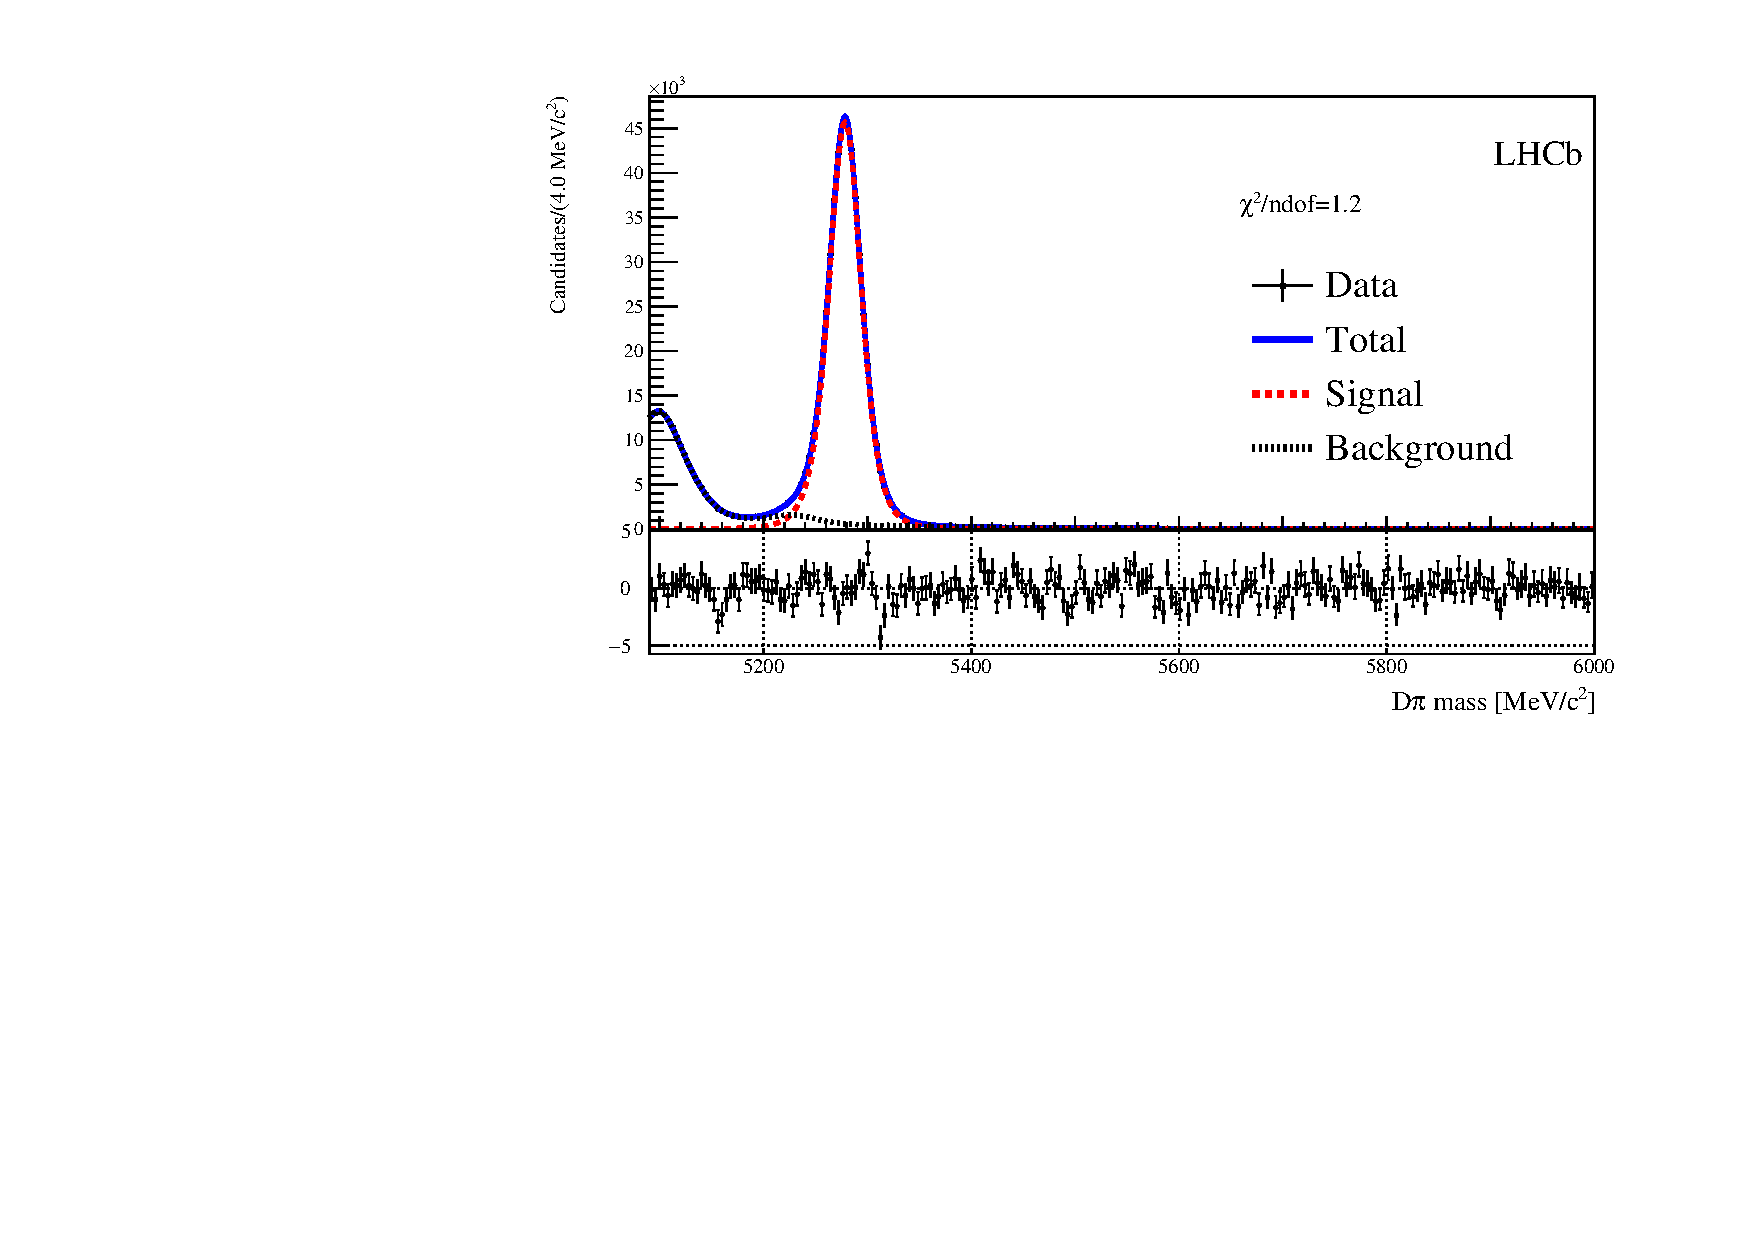
\includegraphics[width=0.7\linewidth]{06Systematics/figs/MDFitPlots_Bd_largeWindow/MDFitForSWeights_BeautyMass_Bd2DPi.pdf}
        \end{center}
        \vspace{-2mm}
        \caption{$\Dmp\pipm$ mass distribution of the $\pi$ sample with the results of Fit B in the large mass window superimposed.}
        \label{fig:FitBWideMass}
\end{figure}

Another test is made by repeating the mass fit with a different strategy:
\begin{itemize}[noitemsep,topsep=0pt]
  \item a $\PIDK<0$ cut (instead of $\PIDK<5$) is applied on the pion PID in order to define the pion sample;
  \item both Fit A and Fit B are performed in the narrow signal region ($[5220,5600]\mevcc$);
  \item during Fit A, only the pion sample is considered (no simultaneous fit in kaon and pion samples is performed);
  \item only $\Bz\to\Dmp\Kpm$ and combinatorial background are considered, whereas all the other physical background are neglected;
  \item the $\Bz\to\Dmp\Kpm$ yield is Gaussian constrained to be $0.0101\pm0.0012$ of the signal yield, based on the selection efficiencies 
    (including the $\PIDK<0$ cut) found on Monte Carlo.
\end{itemize}
The signal and total background yield obtained in this fit are $406\,818\pm674$ and $23\,938\pm266$ respectively.
The projection of the PDF used for Fit A and Fit B in this configuration is shown in Fig.~\ref{fig:MassFitPIDK0}. 
A decay time fit is performed on the resulting sample with \emph{sWeights}
by following the same strategy as reported in Sec.~\ref{sec:datafit}. The correlated discrepancy between the result of this fit and that of the nominal fit is $0.4~\sigma$
and $1.6~\sigma$ for $S_f$ and $S_{\bar f}$ respectively. Given the good level of agreement, and the fact that systematic uncertainties on the PID efficiencies are already considered, no further systematics are assigned.

\begin{figure}[htbp]
        \begin{center}
                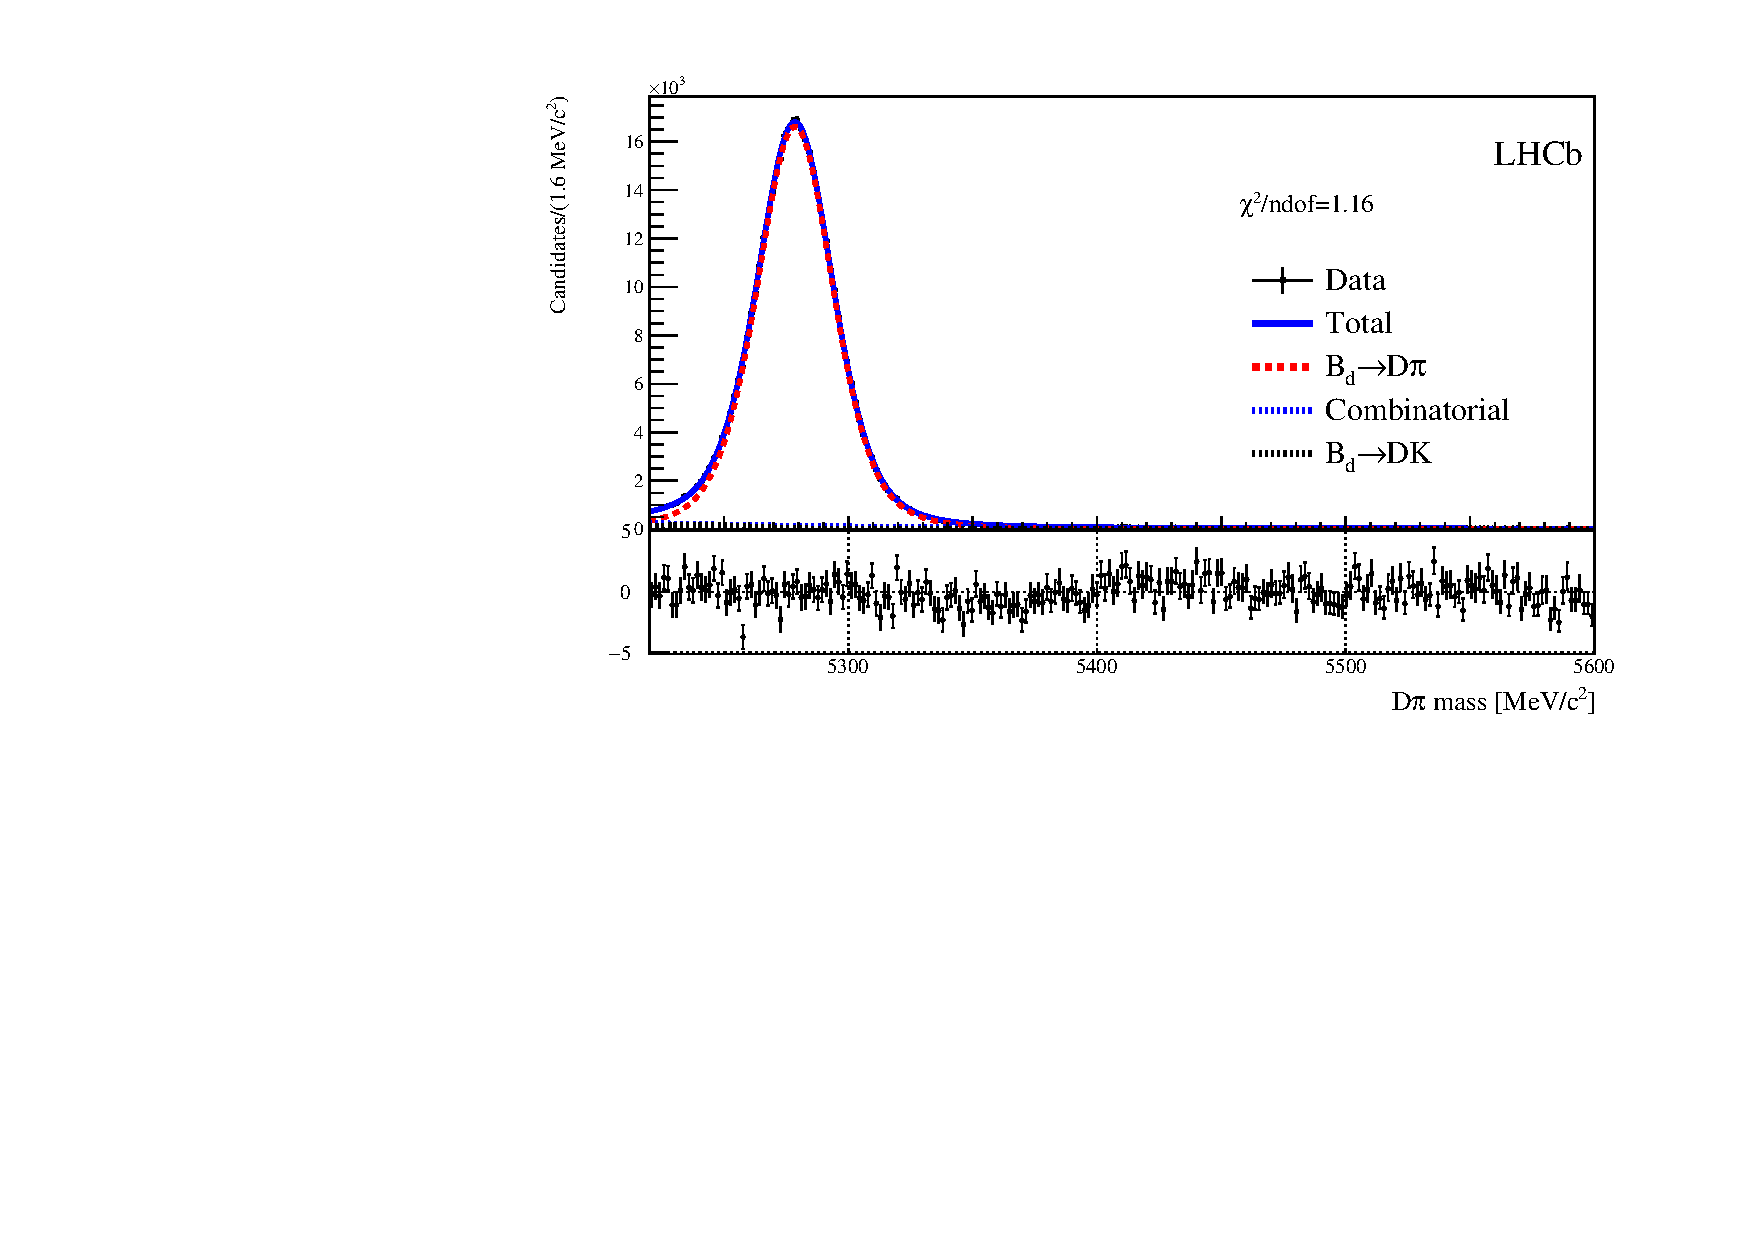
\includegraphics[width=0.49\linewidth]{06Systematics/figs/MDFitPlots_Bd_pidk0/MDFit_BeautyMass_Bd2DPi_withPulls.pdf}
                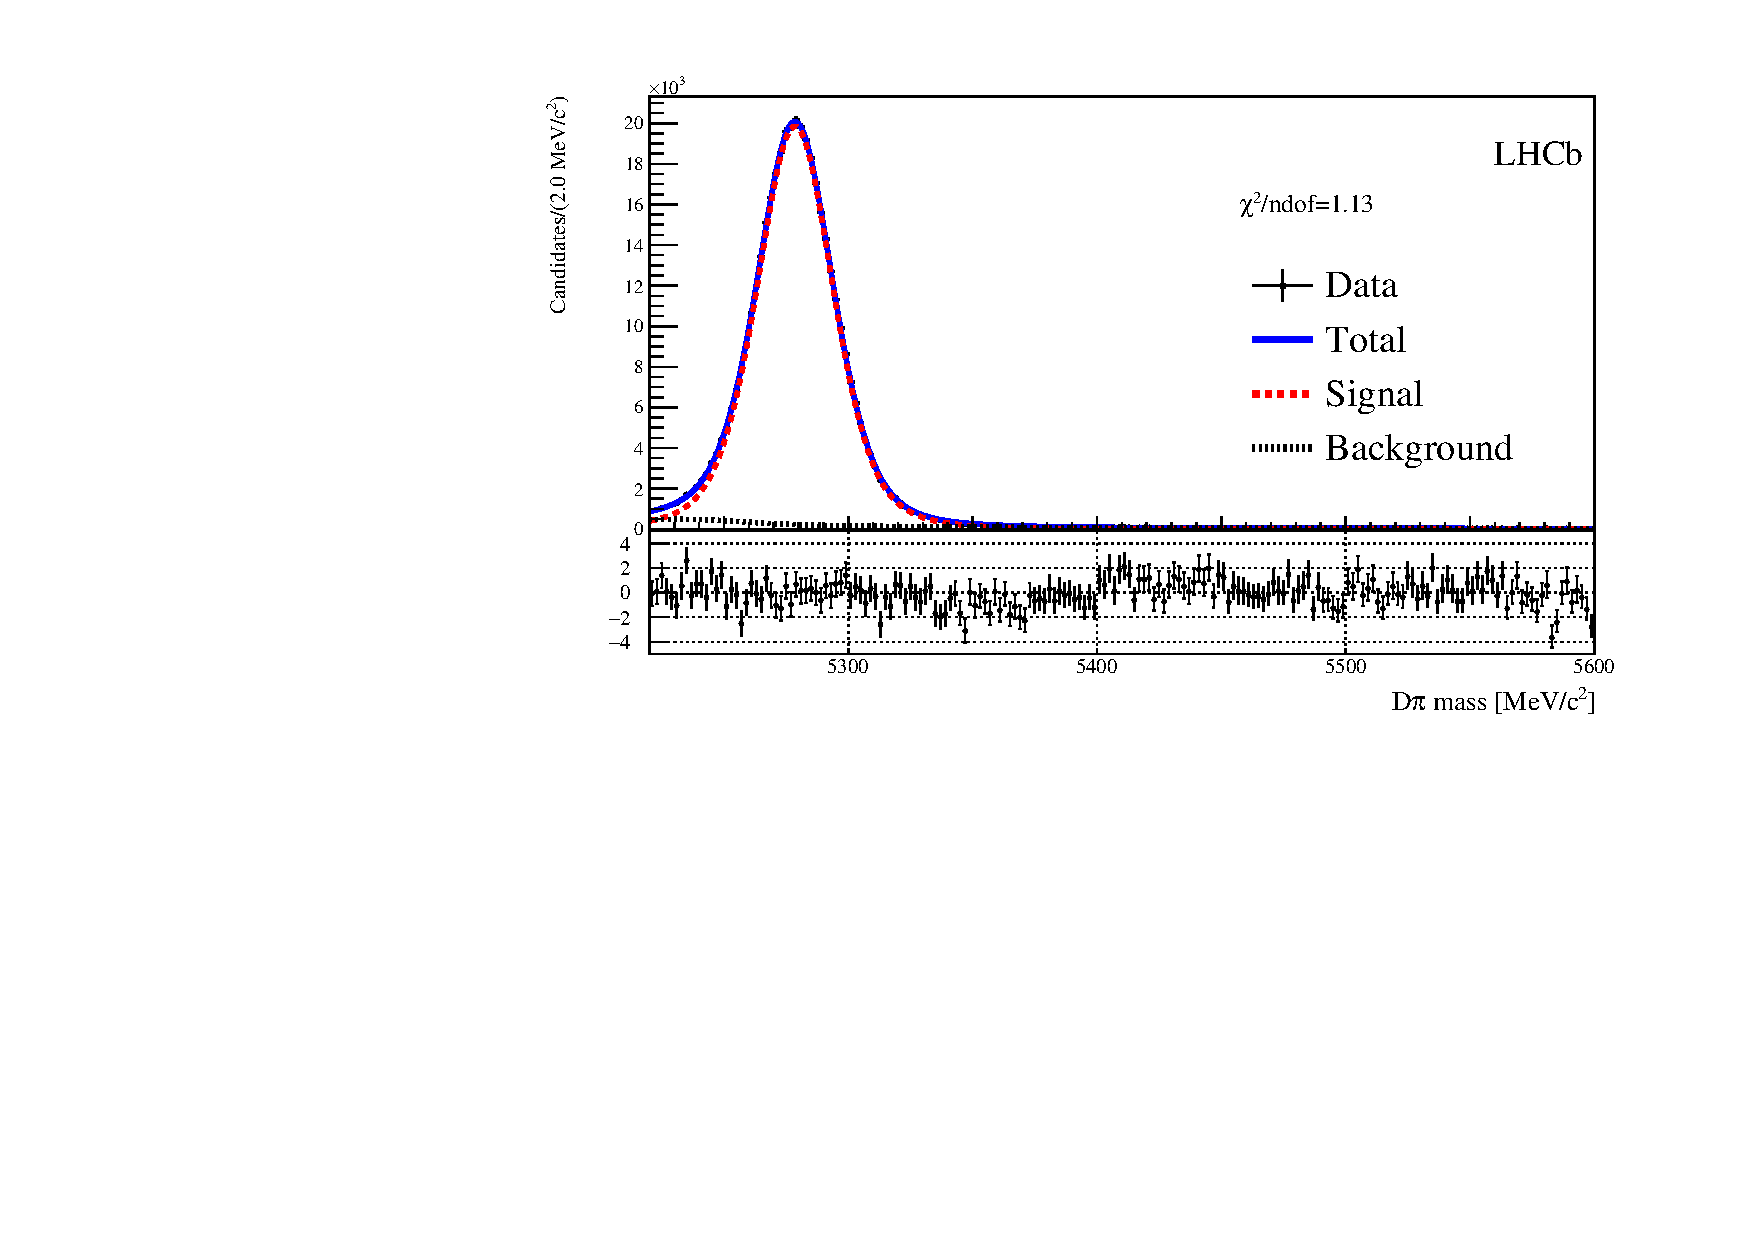
\includegraphics[width=0.49\linewidth]{06Systematics/figs/MDFitPlots_Bd_pidk0/MDFitForSWeights_BeautyMass_Bd2DPi.pdf}
                \end{center}
        \vspace{-2mm}
        \caption{$\Dmp\pipm$ mass distribution of the alternative $\pi$ sample defined by the cut PID$K<0$ on the bachelor pion with the result of Fit A (left) and Fit B (right) superimposed.}
        \label{fig:MassFitPIDK0}
\end{figure}

As additional cross-check, the decay time fit is repeated for $\Bz\to\Dmp\pipm$ candidates restricted in the $[5250,5330]\mevcc$ invariant mass region, very close to
the $\Bz\to\Dmp\pipm$ signal peak position. No \emph{sWeights} are applied on this subsample. 
The correlated disagreement between the result of this fit and that of the nominal fit is $0.2~\sigma$ and $1.3~\sigma$ for $S_f$ and $S_{\bar f}$ respectively. 
Given the good level of agreement, no further systematics are assigned, and the following conclusions are drawn:
\begin{itemize}[noitemsep,topsep=0pt]
  \item the amount of combinatorial and $\Bz\to\Dmp\Kpm$ backgrounds in the signal region is very small,
    and their presence doesn't affect significantly the fitted $S_f$ and $S_{\bar f}$ coefficients as these are compatible with the nominal fit result;
  \item any systematics due to a wrong modelling of signal and/or background PDF in the $\Bz\to\Dmp\pipm$ signal peak region is negligible, since the fitted value obtained from the nominal fit (with \emph{sWeights})
    and this alternative fit (with no mass fit at all) are compatible.
\end{itemize}

